\clearpage

%删去有关向量定义的内容
%完善第二节逻辑：视角转换对理解概念的重要性+实际问题的重要性

\section{线性代数的基本概念和原理}

\subsection{概述：$\mathbb{R}^n$中的线性映射与矩阵}

\subsubsection{引入：横梁弯曲的几何学}

设有一矩形截面横梁$ABCD$，
上面画着一系列平行等距直条纹.
当这根横梁被弯曲成$ABC'D'$时，
直条纹也随之弯曲成平行等距的曲线条纹.
我们在横梁截面上选择很微小的一块方形面积$\mathrm{d} \sigma$来研究，
用浅蓝色方框表示.
这部分材料随着横梁的弯曲，
移动和变形到了深蓝色区域$\mathrm{d} \sigma'$（图\ref{fig:bending}左）.
这片方形区域仍然是很微小的.
因此，处于这片方形区域之内的平行曲线条纹也都是极短的.
根据微分的思想，
这部分曲线可以近似地看成是直线（图\ref{fig:bending}中）.
这说明，
虽然横梁在宏观上弯曲，
但是在微观上，
横梁的任何一点附近都可以近似地看成没有弯曲或扭转，
而是只发生诸如旋转、伸缩等“平直均匀”的运动.

\begin{figure}[H] 
    \centering
    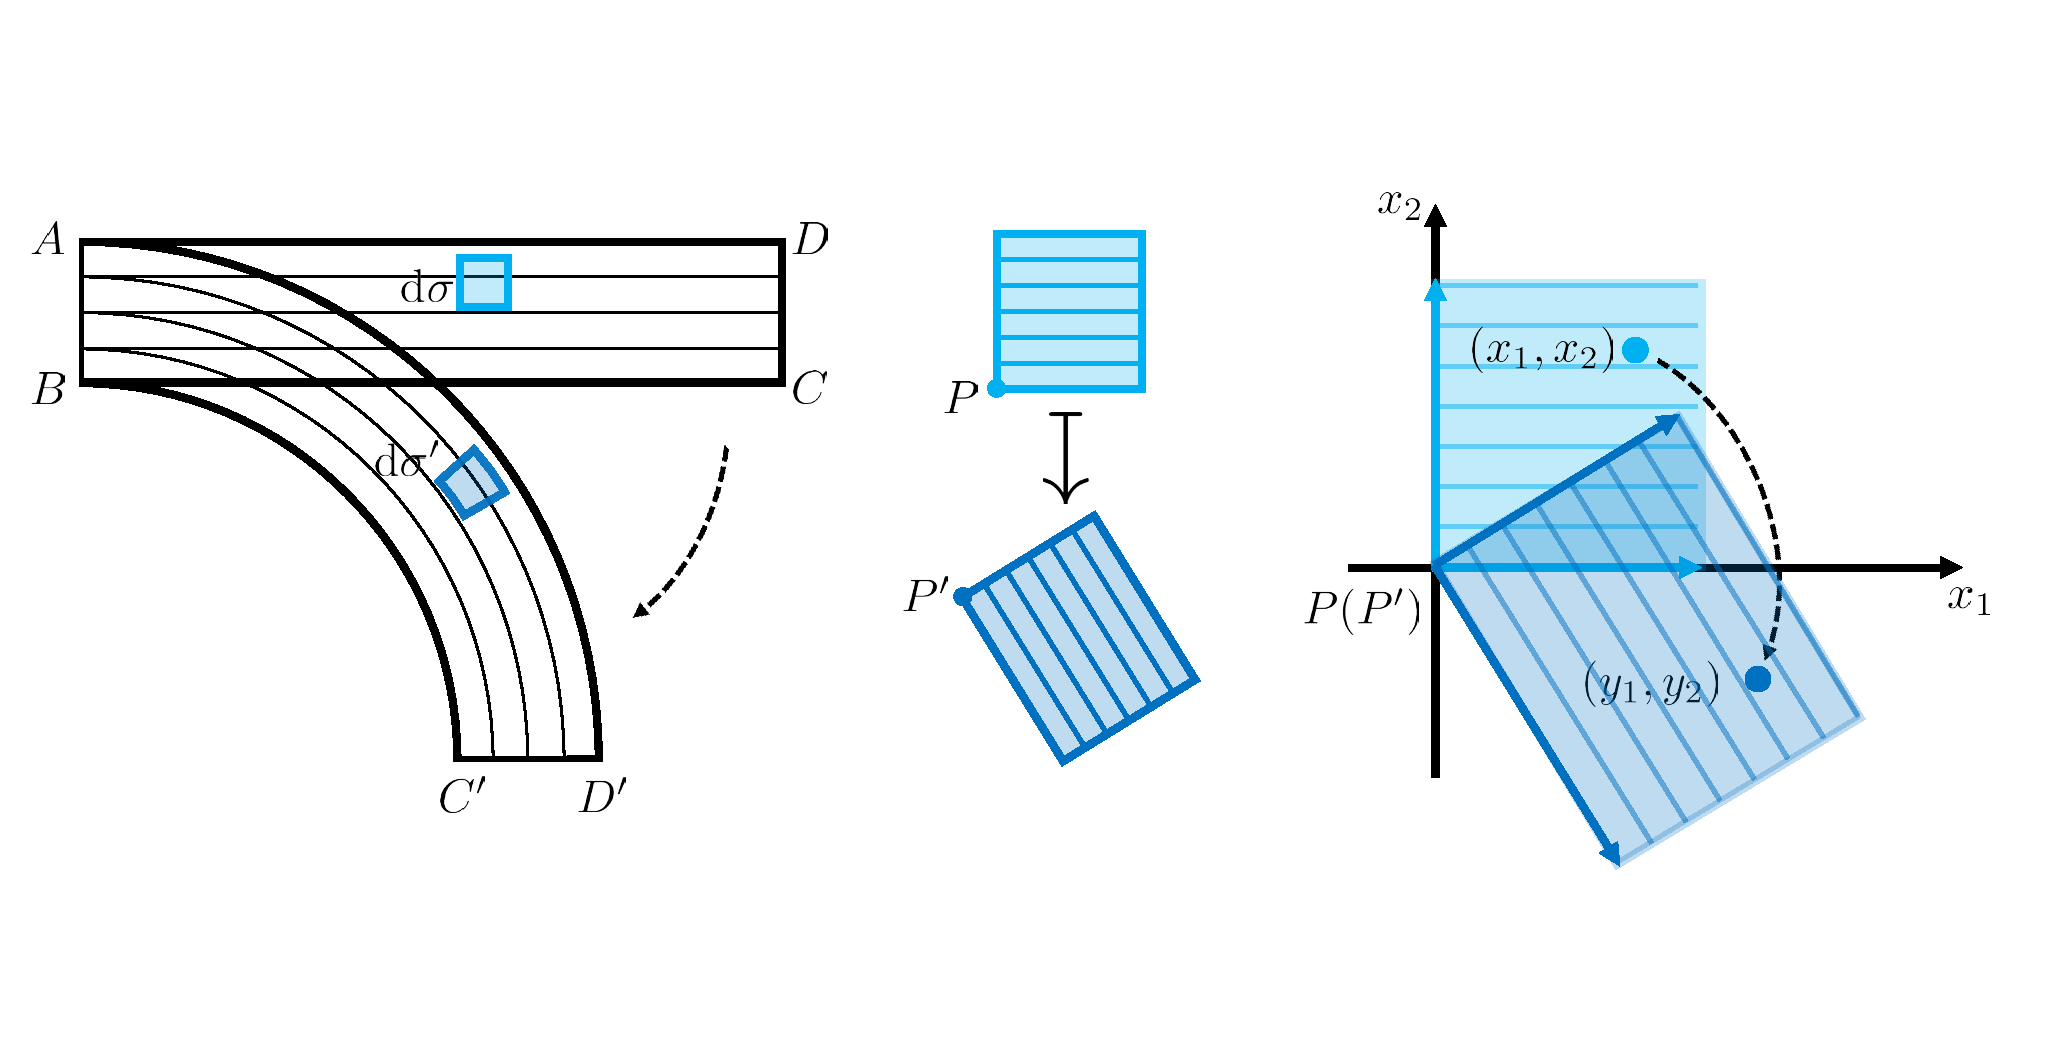
\includegraphics[trim=0 3cm 0 2cm, clip, width=1\textwidth]{fig/fig_bending.pdf}
    \caption{材料变形中的线性映射}
    \label{fig:bending}
\end{figure}

现在用数学语言描述此类运动.
我们将$\d \sigma$左下角的一个物质点标记为$P$，
横梁弯曲后它移动到了$P'$.
我们希望考察$P$点附近微小区域形变的特征，
而非空间位置的移动.
因此，把$\d \sigma$与$\d \sigma'$叠放在一起，
使得$P$与$P'$重合，
然后以$P$为坐标原点建立$\mathbb{R}^n$中的平面坐标系，
横轴和纵轴分别为$x_1$和$x_2$（图\ref{fig:bending}右）.
这样一来，$\d \sigma$中任意一个物质点都获得了一个坐标向量$\bm{x} = (x_1,x_2)$；
而在横梁弯曲后，
该物质点发生位移，
于是在同一个坐标系中获得了另一个坐标向量$\bm{y} = (y_1,y_2)$.
根据前述的讨论，
把向量$\bm{x} = (x_1,x_2)$映为向量$\bm{y} = (y_1,y_2)$的映射满足两个条件：\medskip

\textit{(1)~它保持原点（零向量）不变；}

\textit{(2)~它将等距平行的直线条纹映为等距平行的直线条纹. 
（严谨地说：任意三个共线的点在映射作用后仍然共线，且任意两条共线线段的距离之比在映射作用下保持不变.）} \medskip

上述两个条件给出了\textbf{线性映射}的几何化定义，
它对任何$\mathbb{R}^n \to \mathbb{R}^m$的映射都适用，
称为\textbf{$\mathbb{R}^n$到$\mathbb{R}^m$的线性映射}.
在实际问题中，
我们尤其关心一个空间到自身的线性映射.
就比如在上面的例子中，
平面内物体运动前后的状态变化被描述为$\mathbb{R}^2 \to \mathbb{R}^2$的线性映射，
更一般地，
我们将来会经常遇到
$\mathbb{R}^n \to \mathbb{R}^n$的线性映射，
称其为\textbf{$\mathbb{R}^n$上的线性变换}.

线性映射是线性代数中最重要的研究对象之一.
毫无疑问，
线性映射是各种五花八门的映射中最简单的一种
（例如$\mathbb{R}\to \mathbb{R}$的函数中，
是线性映射的只有线性函数$y=kx$）.
生活和研究中的问题往往不是线性映射那么简单，
但线性代数对此并不是无能为力——
恰恰相反，
我们能通过局部近似的思想把非线性问题近似成线性问题，
把握住问题最重要的特征.
刚才介绍的材料变形问题就是一个典型的例子.

\subsubsection{$\mathbb{R}^2$上的线性变换}

在线性代数中，
我们要研究任意维度的向量，
也就会涉及到高维的线性映射.
因此，高维的人类学习线性代数可能更有优势.
但是，
高维的问题总可以看成低维情形的推广.
作为$3$维的人类，
我建议大家先通过具体例子和图像，
明白$\mathbb{R}, \mathbb{R}^2$和$\mathbb{R}^3$空间上的线性变换是怎么回事.
其中，
以$\mathbb{R}^2$上的线性变换最为重要.
因为它对于$3$维人类来说比较简单，
却能带给我们足够多的规律.

接下来，我们来研究$5$类$\mathbb{R}^2$上典型的线性变换，
它们各自对应一种具体的运动形式.
图像下方列出了线性变换所对应的公式，
即$\bm{y} = (y_1,y_2)$关于$x_1,x_2$的表达式（图\ref{fig:R2}）.
当然，同学们可以自行验证这些表达式是正确的，
而且符合线性映射的定义.
不过这里暂且无意于做严格的数学推导，
让我们先对线性变换“长什么样”有一个直观的认识：\medskip

(1)~\textbf{旋转}：如图\ref{fig:R2}(1)所示.
整个平面绕原点$O$逆时针旋转$\theta$角.


(2)~\textbf{反射}：如图\ref{fig:R2}(2)所示.
整个平面以纵轴$x_2$轴为旋转轴，翻转$180 ^\circ$.
也可以理解为：平面上的每个向量$\bm{x} = (x_1,x_2)$以$y$轴为“镜面”，
映照到与之对称的$\bm{y} = (y_1,y_2)$处.

(3)~\textbf{剪切}：如图\ref{fig:R2}(3)所示.
整个平面沿着平行于横轴$x_1$轴的方向发生错动，倾斜$\theta$角.

(4)~\textbf{伸缩}：如图\ref{fig:R2}(4)所示.
整个平面沿$x$轴横向伸缩$k_1$倍，沿$y$轴纵向伸缩$k_2$倍.

(5)~\textbf{平行投影}：如图\ref{fig:R2}(5)所示.
当太阳高度角为$\theta$时，
向量$(x_1,x_2)$被平行光照射到$x$轴上，其影子的坐标是$(y_1,y_2)$.
也可以理解为：
整个平面沿$\theta$倾斜角方向被均匀地“拍扁”到$x$轴上.\medskip

\begin{figure}[H] 
    \centering
    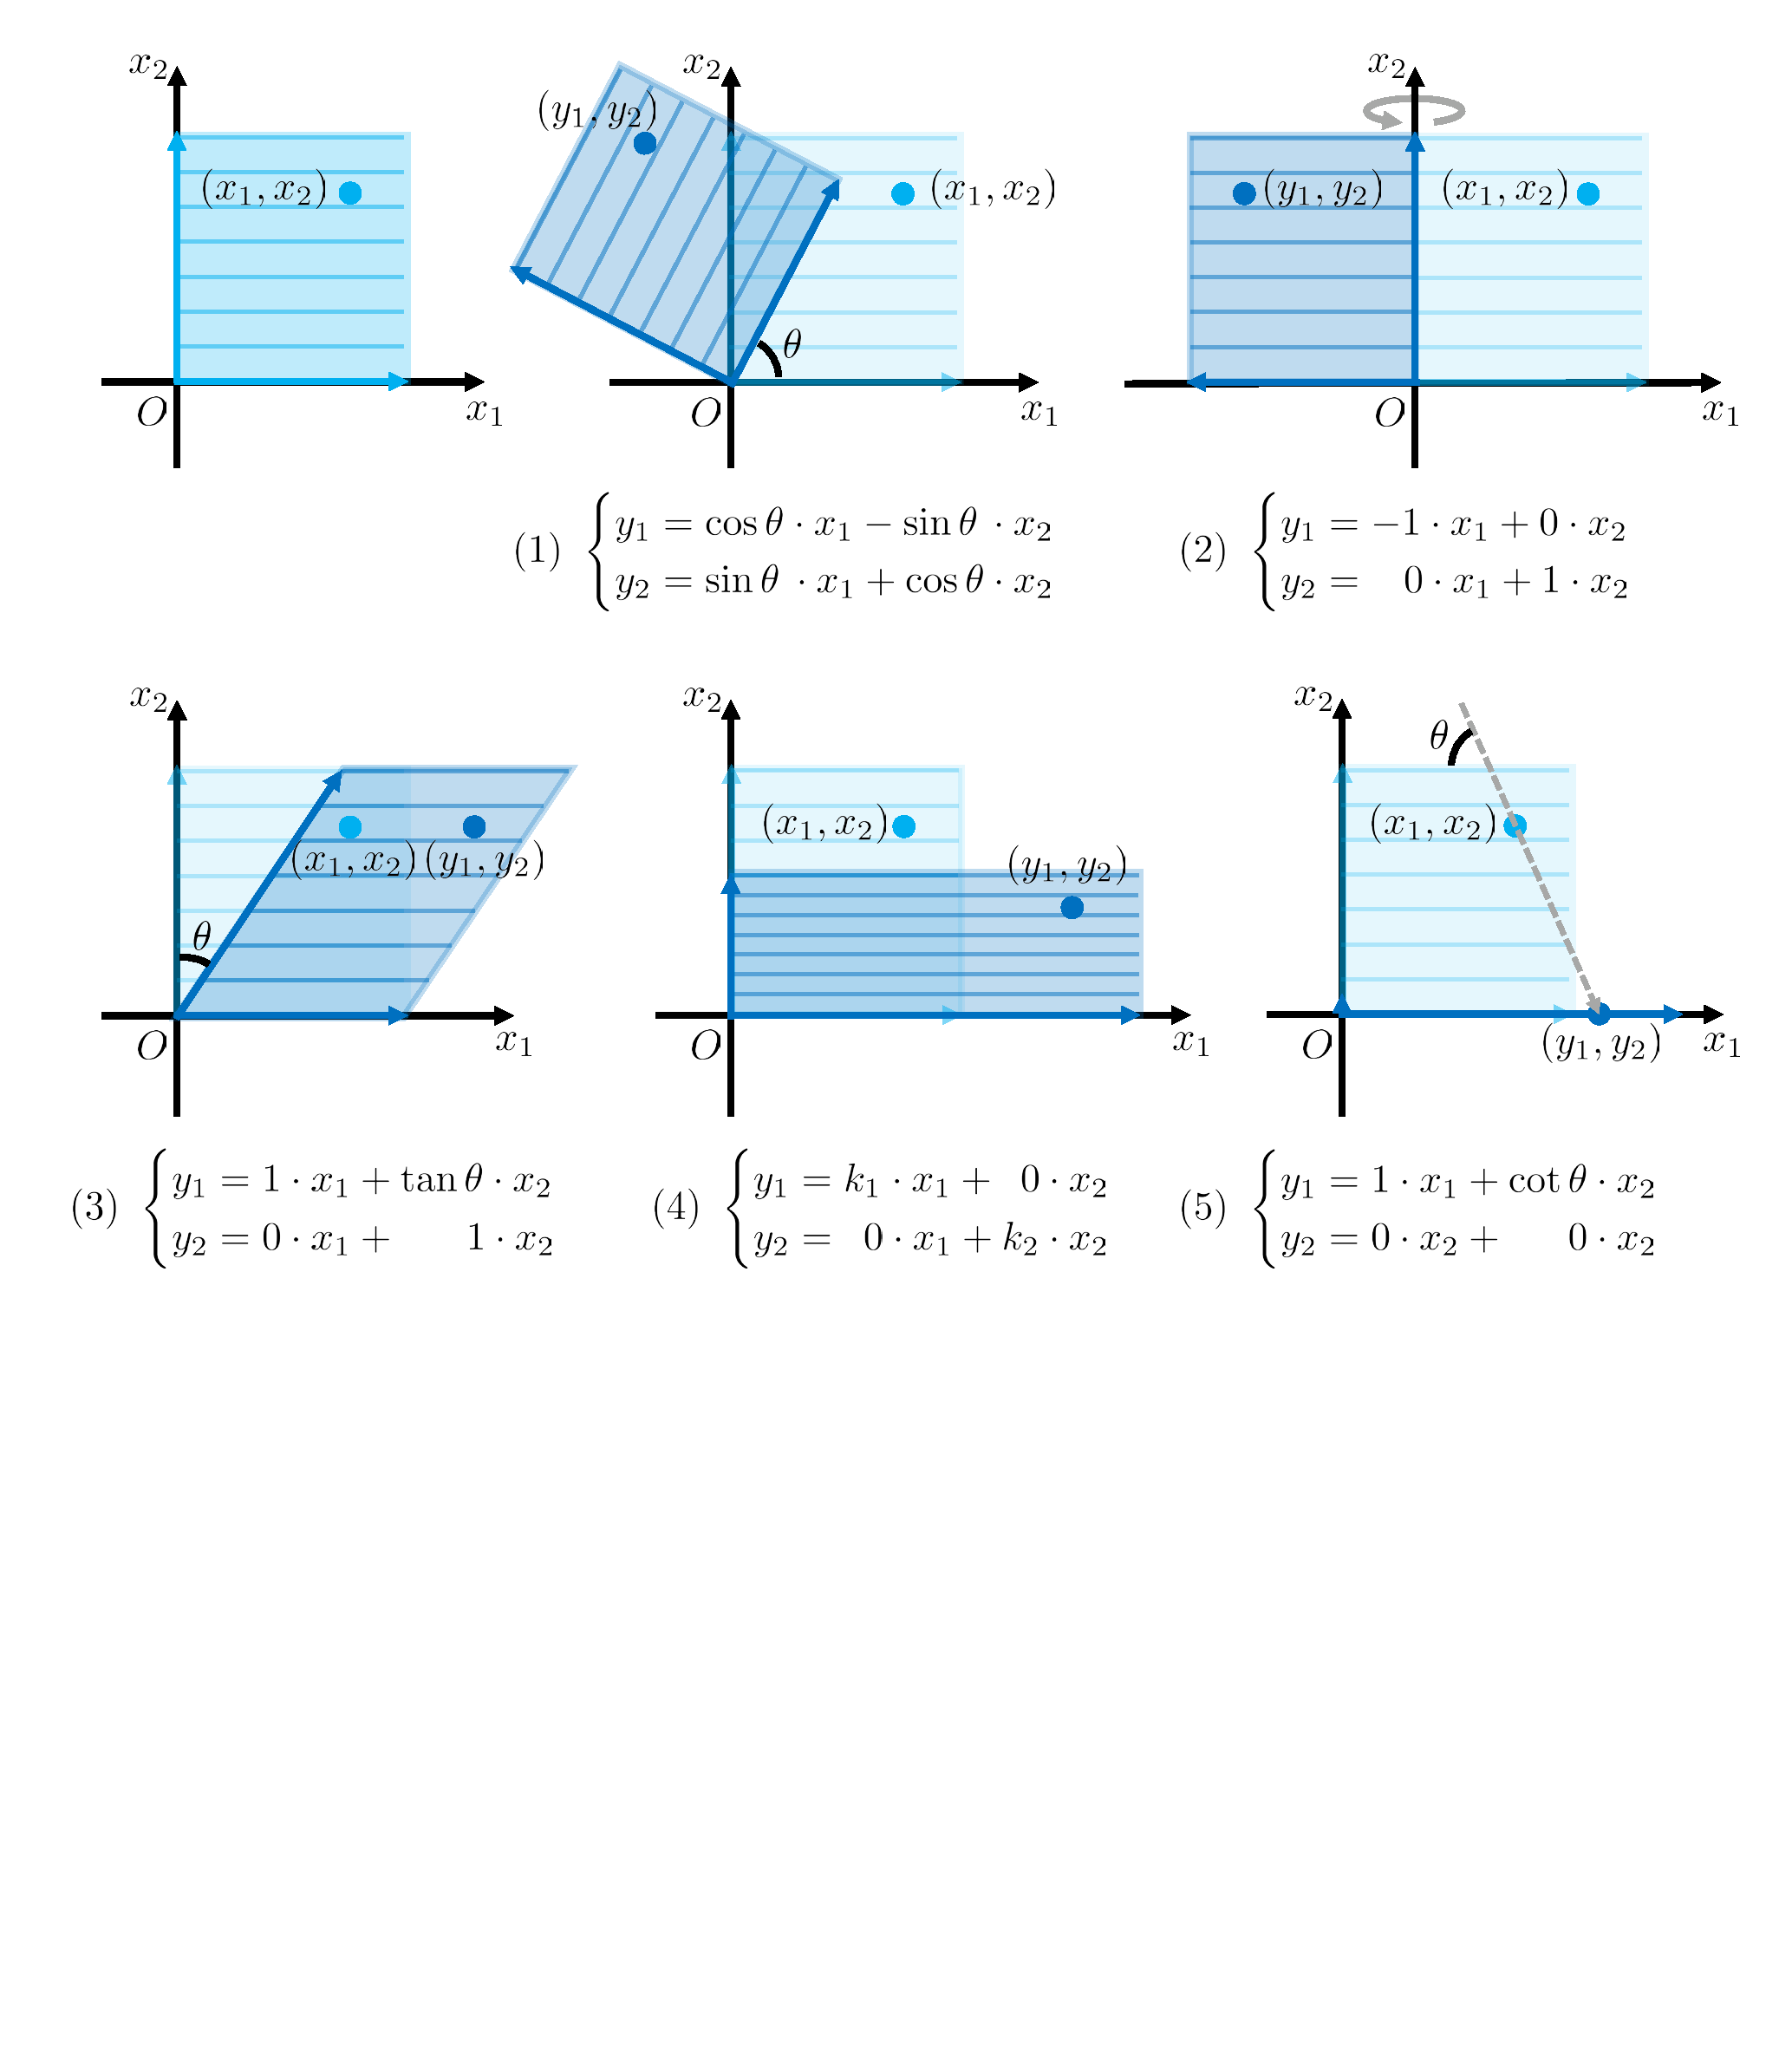
\includegraphics[trim=0 15cm 0 0, clip, width=1\textwidth]{fig/fig_R2_2.pdf}
    \caption{5类基本的线性变换~~(1)旋转；(2)反射；(3)剪切；(4)伸缩；(5)平行投影.}
    \label{fig:R2}
\end{figure}

从表达式上看，
这$5$类线性变换有一个明显的共同点，
那就是它们都可以用\textbf{线性方程组}表示.
也就是说，
$\bm{y} = (y_1,y_2)$的表达式中仅含有$x_1,x_2$的一次项，
为$x_1,x_2$的一次齐次多项式.
事实上，用线性方程组表示的映射都是线性映射，
而且凡是线性映射都能用线性方程组表示.
因此，
完全可以把线性映射“望文生义”地理解为“\textbf{由线性方程组所表示的映射}”.
于是，我们写出$\mathbb{R}^2$上的线性变换的一般形式：\medskip
\begin{eq1}
    \begin{cases}
        y_1 = a_{11} \cdot x_1 + a_{12} \cdot x_2\\[2pt]
        y_2 = a_{21} \cdot x_1 + a_{22} \cdot x_2
    \end{cases} \end{eq1} 

在此基础上可以进一步证明，
映射$A$是线性映射当且仅当它满足两个“线性”性质：

(1)~$A\bm{x}_1 + A\bm{x}_2 = A(\bm{x}_1 + \bm{x}_2)$；

(2)~$kA\bm{x} = A(k\bm{x})$.

到目前为止，
我们对于线性映射的概念已经提出了三种解释方法.
平行等距直条纹的解释方法直观性很强，
但不便于操作.
线性方程组的观点是联系理论与应用的桥梁.
而两种线性性质的表述则比较简洁和抽象，
能够体现线性的本质，
因此我们将其作为线性映射的真正定义.
三种表述的等价性将在习题中证明.

线性变换是一种映射，
而映射是可以复合的.
例如，
记线性变换$A$是“沿$x_1$轴方向伸缩$k$倍”，
记线性变换$B$是“绕$O$顺时针旋转$\theta$角”.
那么，“先沿$x_1$轴方向拉长$k$倍再绕$O$顺时针旋转$\theta$角”也是$\mathbb{R}^2$上的一个线性变换，
记为$BA$（注意映射的复合是从右往左写的）.
不妨动笔计算一下它的表达式:
设任意的$\mathbb{R}^n$中的向量$\bm{x} = (x_1,x_2)$，
它经$A$变换成为向量$\bm{y} = (y_1 , y_2)$，
再经$B$变换成为向量$\bm{z} = (z_1, z_2)$.
由$A$和$B$的公式可以写出：
\begin{eq1}
    \begin{cases}
        y_1 = k x_1 \\[2pt]
        y_2 = x_2
    \end{cases}
    ~~~
    \text{和}
    ~~~~~~
    \begin{cases}
        z_1 = ~~\cos \theta \cdot y_1 + \sin \theta \cdot y_2 \\[2pt]
        z_2 = -\sin \theta \cdot y_1 + \cos \theta \cdot y_2
    \end{cases} \end{eq1} 

通过代入，
直接得到$(z_1,z_2)$关于$(x_1,x_2)$的表达式，
也就是复合映射$BA$的公式：
\begin{eq1}
    \begin{cases}
        z_1 = ~~k \cos \theta \cdot x_1 + \sin \theta \cdot x_2 \\[2pt]
        z_2 = - k \sin \theta \cdot x_1 + \cos \theta \cdot x_2 
    \end{cases} \end{eq1}

这仍然是一个线性方程组，
表明$BA$确实是线性变换.
这个计算过程也让我们领悟到，
线性表达式与线性表达式的复合一定还是线性表达式，
表明\textbf{任何线性变换的复合仍然是线性变换}（\textbf{任何线性映射的复合仍然是线性映射}）.
反过来说，
任何线性变换都可以分解成若干个比较简单的线性变换的复合.
这就好比是拧魔方，
只要以合适的顺序执行几种基本的转动操作，
就可以产生千变万化的状态.
从几何的角度来说，
\textbf{旋转、反射、剪切、伸缩和平行投影}
就是线性变换中最基本的操作.
它们的运动形式易于理解，
可以推广到高维，
而且在实际问题中也随处可见它们的身影.
因此在之后的学习中，
可以把这$5$类基本操作当作模板.

\begin{figure}[H] 
    \centering
    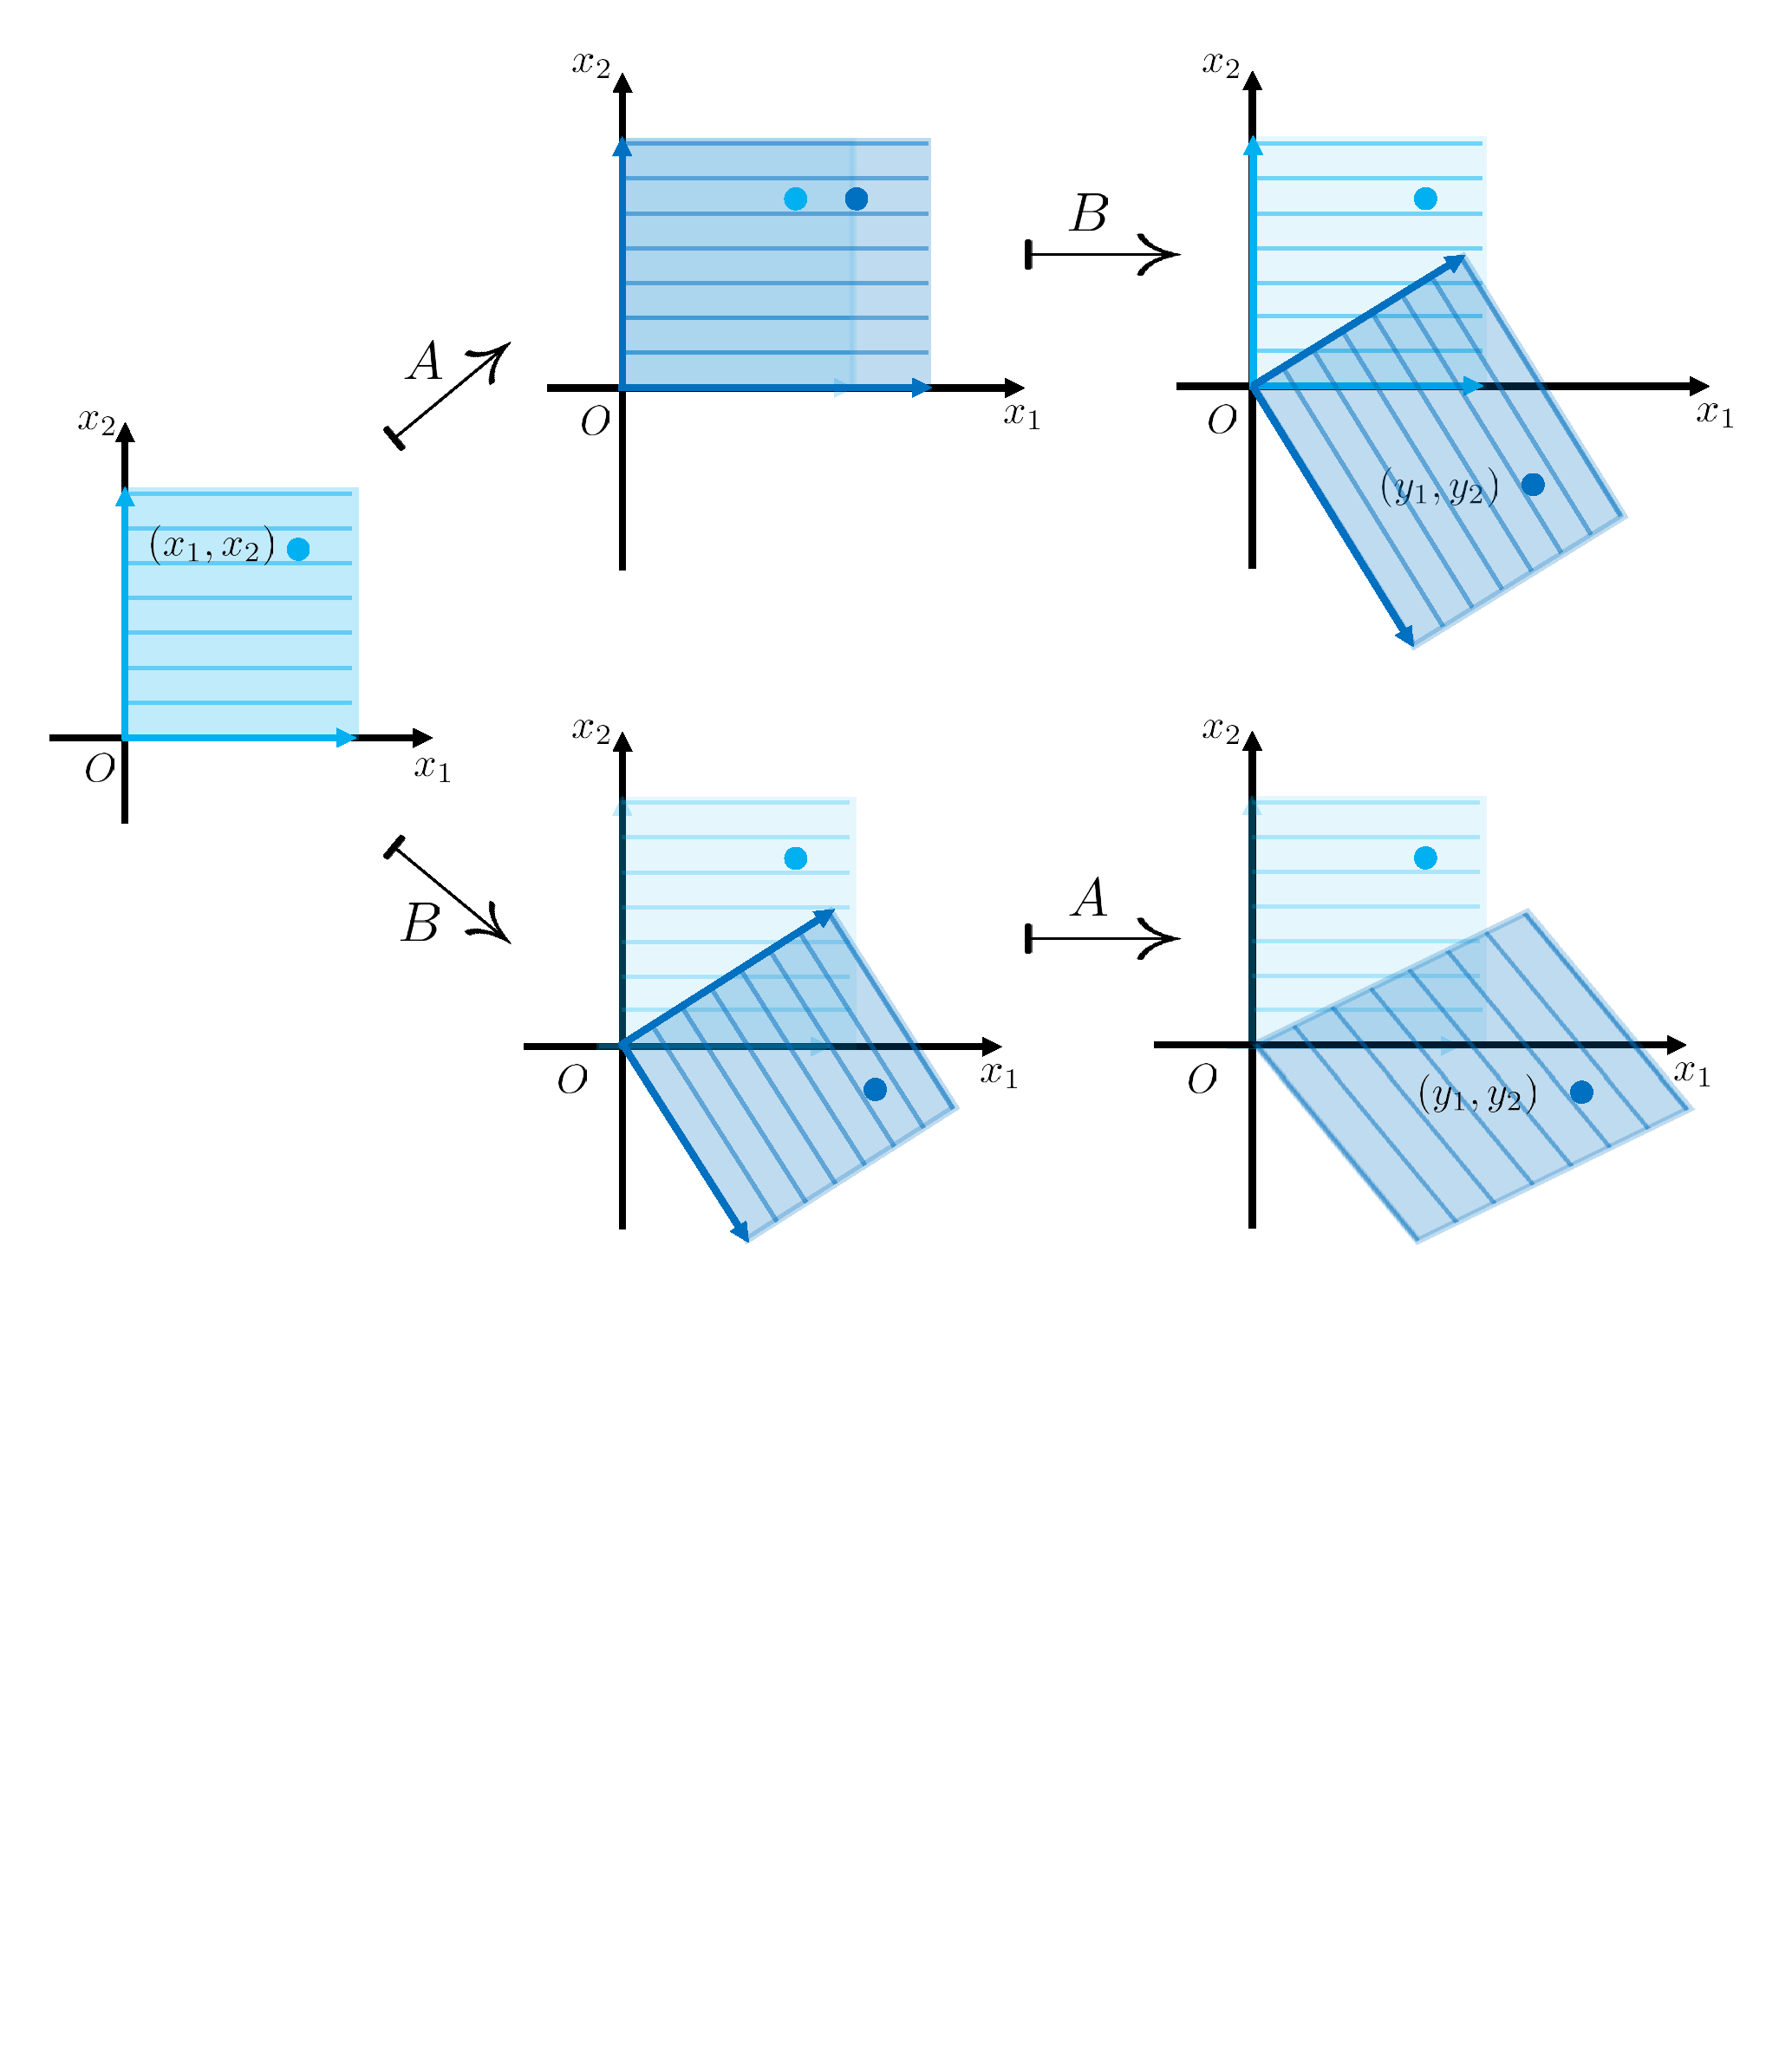
\includegraphics[trim=0 15cm 0 0, clip, width=0.8\textwidth]{fig/fig_BAAB.pdf}
    \caption{线性映射$A$与$B$的复合顺序不可交换}
    \label{fig:BAAB}
\end{figure}

说到映射的复合，
必须关注它们的顺序.
线性变换也是如此.
一般来说，
两个线性变换以不同的先后顺序复合，
所合成的线性变换是不同的.
例如，“先沿$x_1$轴方向拉长$k$倍再绕$O$顺时针旋转$\theta$角”
与
“先绕$O$顺时针旋转$\theta$角再沿$x_1$轴方向拉长$k$倍”
就是不同的，
即$AB \ne BA$（图\ref{fig:BAAB}）.




对于映射，
我们还会谈及\textbf{单射}、\textbf{满射}和\textbf{双射}的概念.
双射是\textbf{可逆映射}，
可以定义其\textbf{逆映射}.
一个映射与其逆映射复合的结果是\textbf{恒等映射}（即“什么都不做”）.
这些概念放在$\mathbb{R}^2$上线性变换的语境中如何理解？
让我们回到$5$类基本操作上.
不难发现：\medskip

(1)~旋转变换是双射.
逆时针旋转$\theta$角的逆变换是顺时针旋转$\theta$角.

(2)~反射变换是双射. 它是自身的逆变换.

(3)~剪切变换是双射. 朝某个方向错动倾斜$\theta$角的逆变换是朝反方向错动倾斜相同角度.

(4)~伸缩变换是双射. 沿$x_1,x_2$轴分别伸缩$k_1,k_2$倍的逆变换是沿$x_1,x_2$轴分别伸缩$\frac{1}{k_1},\frac{1}{k_2}$倍.\medskip

而(5)~平行投影与其他$4$类格格不入.
以投影到$x_1$轴为例.
$\mathbb{R}^2$中任何两个平行于阳光方向排列的点，
其“影子”是重合的，即它们在平行投影下的像是同一个，因此平行投影不是单射；
另外，$\mathbb{R}^2$上只要不在$x$轴上的点都没有平行投影的原像，
因此它也不是满射.
综上，
平行投影既不是单射也不是满射，
更不是双射，
不存在逆映射.
从直观上，
这是因为一个$2$维物体被“压缩”成$1$维时损失了信息.
一个物体即使被旋转、反射、剪切或伸缩，
我们总还能认出它原本的模样，
但是仅凭影子却无法还原出这个物体.
那么，如何计算一个线性变换是否可逆？
如果可逆，如何计算出它的逆变换？
对于$\mathbb{R}^2$上的线性变换，
无非是要从$(y_1,y_2)$反解出$(x_1,x_2)$来：
\begin{eq1}
    \begin{cases}
        y_1 = a_{11} \cdot x_1 + a_{12} \cdot x_2 \\[2pt]
        y_2 = a_{21} \cdot x_1 + a_{22} \cdot x_2
    \end{cases}
    \Longleftrightarrow ~~
    \begin{cases}
        x_1 =  \frac{a_{22}}{a_{11}a_{22} - a_{12}a_{21}} \cdot y_1 
        + \frac{-a_{12}}{a_{11}a_{22} - a_{12}a_{21}} \cdot y_2 \\[12pt]
        x_2 = \frac{-a_{21}}{a_{11}a_{22} - a_{12}a_{21}} \cdot y_1 
        + \frac{a_{11}}{a_{11}a_{22} - a_{12}a_{21}} \cdot y_2
    \end{cases}  \end{eq1} 
其中要求分母$a_{11}a_{22}-a_{12}a_{21} \ne 0$，
否则，不存在逆变换.
这些计算结果的意义，
我们稍后再深入探究，
先来细品一下我们刚刚从计算过程中获得的洞见：
\textbf{求解线性变换的逆变换就是求解线性方程组的问题.}
刚才我们计算了$\mathbb{R}^2$上线性变换的逆变换，
实际上就是小学生级别的二元一次方程组问题.

这问题看似简单，
却提出了新的挑战：
假如要写出$\mathbb{R}^3$上线性变换的逆变换的一般公式，
用$9$个系数$a_{ij}$表示，
毫无疑问是很冗长的，
以至于这个版面会放不下.
变量数如果更多就更不必说了.
对常人来说，
即使耐心十足地做出了全部的计算，
最终也不过是迷失在繁杂冗长的表达式中，
得不到任何更进一步的规律.
如果有一套更好的数学体系和符号系统，
不仅能方便计算，
更能我们把有限的智商从计算中节省出来，
用于分析更加深刻的问题.

在小学阶段，
我们都曾学过“鸡兔同笼”的问题.
我们将鸡与兔的数量抽象成“未知量”的概念，
以字母符号$x$和$y$代之，
这正是“代数”一词的本意.
利用未知量和等量关系建立线性方程组，
能使问题标准化、清晰化、一般化.
站在这个高度往回看，
诸如“让所有兔子抬起两只脚站立起来”这种取巧的算术解法就显得过时了.
今天，我们早已习惯了“未知量”的概念，
习惯了使用字母符号在花括号中列出一条一条的线性方程，
是否想过这些概念和符号也会新的需要而“过时”？
当我们认识到线性方程组背后有“线性映射”这样一个更深刻的概念时，
就已经来到了一个新领域的边缘.
但要真正推开它的大门，
我们必须要问：
用什么方法能更简单地表示线性映射？
该用什么样的符号来“代”它？
使用这套新符号能挖掘出什么更深刻的结论？


\subsubsection{$\mathbb{R}^n$中线性映射的矩阵表示}

线性代数通过引入\textbf{矩阵}和\textbf{矩阵乘法}的规则，
巧妙地把大量线性运算“集成”起来，
让我们得以具体地把握任何维度的线性映射的性质.
为了方便解释，
我们先用“传统办法”写出$\mathbb{R}^n \to \mathbb{R}^m$的线性映射的一般公式.
它把$\mathbb{R}^n$中的向量$\bm{x} = (x_1 , x_2 , \cdots ,x_n)$
映成
它把$\mathbb{R}^m$中的向量$\bm{y} = (y_1 , y_2 , \cdots ,y_m)$：
\begin{eq1}
    \begin{cases}
        y_1 = a_{11} x_1 + a_{12}x_2 + \cdots + a_{1n} x_n \\[2pt]
        y_2 = a_{21} x_1 + a_{22}x_2 + \cdots + a_{2n} x_n \\[2pt]
        ~\vdots \\[2pt]
        y_m = a_{m1} x_1 + a_{m2}x_2 + \cdots + a_{mn} x_n 
    \end{cases} \end{eq1}

这是一个包含$n$个分量，$m$条方程所构成的线性方程组.
在线性代数中，
我们一般愿意把它写成更紧凑的矩阵形式：
\begin{eq1}
    \begin{pmatrix}
        y_1 \\[2pt] y_2 \\[2pt] \vdots \\[2pt] y_m
    \end{pmatrix}
    =
    \begin{pmatrix}
        a_{11} & a_{12} & \cdots & a_{1n} \\[2pt]
        a_{21} & a_{22} & \cdots & a_{2n} \\[2pt]
        \vdots & \vdots & \ddots & \vdots \\[2pt]
        a_{m1} & a_{m2} & \cdots & a_{mn}
    \end{pmatrix}
    \begin{pmatrix}
        x_1 \\[2pt] x_2 \\[2pt] x_3 \\[2pt] \vdots \\[2pt] x_n
    \end{pmatrix} \end{eq1}

其中，
方程组的$mn$个系数$a_{ij} ~(1 \le i \le m,~ 1 \le j \le n)$按方程组中的横竖位置关系排列成了一个数表，称为\textbf{矩阵}.
每个$a_{ij}$都称为矩阵的\textbf{元素}.
它有两个下指标$i$和$j$，
表示该元素处在矩阵的第$i$行，第$j$列.
因此，$i$和$j$分别称为\textbf{行指标}和\textbf{列指标}.
在习惯上，用大写字母来代表矩阵，
也可以用矩阵元素来代表矩阵.
比如，可以用如下的记号指代矩阵：
\begin{eq1}
    A = (a_{ij}) = 
    \begin{pmatrix}
        a_{11} & a_{12} & \cdots & a_{1n} \\[2pt]
        a_{21} & a_{22} & \cdots & a_{2n} \\[2pt]
        \vdots & \vdots & \ddots & \vdots \\[2pt]
        a_{m1} & a_{m2} & \cdots & a_{mn}
    \end{pmatrix} \end{eq1} 

若想强调这个矩阵是一个$m \times n$矩阵（即$m$行$n$列的矩阵），
可以将矩阵的行列数也标记在下指标位置，
如$A_{m \times n},~(a_{ij})_{m \times n}$.
本例中，矩阵$A$是由线性方程组的系数组成的. 
这样的矩阵称为线性方程组的\textbf{系数矩阵}.

在刚刚的矩阵表达式中，
$n$维向量$\bm{x} = (x_1 , x_2 , \cdots ,x_n)$和$m$维向量$\bm{y} = (y_1 , y_2 , \cdots ,y_m)$被竖起来写.
就形式而言，
它们也可以分别视为$n \times 1$的矩阵和$m \times 1$的矩阵.
这样的矩阵称为\textbf{列向量}.
类似地，
横过来写的向量就称为\textbf{行向量}.
在矩阵$A$中，
每一列都可以看成一个列向量，
把所有这些列向量称为这个矩阵的\textbf{列向量组}；
每一行都可以看成一个行向量，
把所有这些行向量称为这个矩阵的\textbf{行向量组}.
如果你只把矩阵$A$看成$mn$个数排列在一起，
这种观点是浮于表面的；
把矩阵$A$看成$m$个行向量（$n$个列向量）“集成”在一起的行（列）向量组，
则是一种更好的理解.

带着这种理解，
我们来了解矩阵运算的规则
（假定同学们已经熟悉了向量的加法、数乘和点乘规则）：
\medskip

(1)~两个相同尺寸的矩阵$A_{m \times n} = (a_{ij})_{m \times n}$和$B_{m \times n} = (b_{ij})_{m \times n}$可以做\textbf{矩阵加法}：
$A+B = (a_{ij} + b_{ij})_{m \times n}$.
也就是说，
两个矩阵做加法就是把对应位置的元素相加，
也可以理解为每个行（列）向量分别对应相加.

(2)~任意实数$k$可以对矩阵$A_{m \times n} = (a_{ij})_{m \times n}$做\textbf{数乘}：
$kA = (ka_{ij})_{m \times n}$.
也就是说，
实数$k$乘矩阵的结果就是把矩阵的每个元素都乘$k$，
也可以理解为把这个矩阵的每个行（列）向量都用$k$数乘.

(3)~一个$m \times n$矩阵$A_{m \times n} = (a_{ij})_{m \times n}$
和一个$n \times s$矩阵$B_{n \times s} = (b_{ij})_{m \times n}$
\medskip 可以做\textbf{矩阵乘法}：
\medskip
$AB = ( \sum_{k=1}^{n} a_{ik}b_{kj})_{m \times s}$.
也就是说，$AB$的第$i$行第$j$的元素是$A$的第$i$个行向量与$B$的第$j$列个列向量进行点乘得到的数，
结果得到一个$m \times s$矩阵.
特别地，一个$m \times n$矩阵$A$和一个$n \times 1$列向量$\bm{x}$做矩阵乘法，
结果是一个$m \times 1$列向量$\bm{y}$.
它的第$i$个分量是$A$的第$i$个行向量与$\bm{x}$的点乘.
\medskip

可以看出，
矩阵的各种运算无非是在批量地进行向量运算.
懂得了矩阵运算的方法之后，
让我们重新审视线性映射的矩阵表达式
（注意这是一个矩阵乘法算式）：
\begin{eq1}
    \begin{pmatrix}
        y_1 \\[2pt] y_2 \\[2pt] \vdots \\[2pt] y_m
    \end{pmatrix}
    =
    \begin{pmatrix}
        a_{11} & a_{12} & \cdots & a_{1n} \\[2pt]
        a_{21} & a_{22} & \cdots & a_{2n} \\[2pt]
        \vdots & \vdots & \ddots & \vdots \\[2pt]
        a_{m1} & a_{m2} & \cdots & a_{mn}
    \end{pmatrix}
    \begin{pmatrix}
        x_1 \\[2pt] x_2 \\[2pt] x_3 \\[2pt] \vdots \\[2pt] x_n
    \end{pmatrix} 
    ~~
    \Longleftrightarrow
    ~~
    \bm{y} = A \bm{x}
    \end{eq1}

这个写法有个显著的优点，
就是将输入向量$\bm{x}$，
输出向量$\bm{y}$与系数$a_{ij}$
完全分离开来，
写成形式上很干净的乘法算式$\bm{y} = A \bm{x}$.
其中，
系数矩阵$A$的元素完全由线性变换所决定.
一个系数矩阵$A$通过表达式$\bm{y} = A \bm{x}$也唯一确定了一个线性映射.
因此，
可以说\textbf{矩阵就是线性映射，线性映射就是矩阵}.
我们在前三章中将不区分线性映射与矩阵的记号，
都用大写字母表示.

在线性代数中，
我们习惯把向量$\bm{x}$当作列向量.
但是在书写行内公式时列向量
$\begin{pmatrix}
    x_1 \\[-6pt]
    x_2 \\[-6pt]
    \vdots \\[-6pt]
    x_n
\end{pmatrix}$
占的空间太大，
显得极不方便.
因此，
我们也会把列向量写作$(x_1 , x_2 , \cdots , x_n)^T$，
其中$T$是转置符号，
代表矩阵的行指标与列指标互换.
因此，
行向量的转置当然就是相应的列向量，
而$\bm{x}^{T}$默认是代表行向量.
对于一般的$m \times n$矩阵$A$
也可以取转置得到相应的$n \times m$矩阵$A^T$.
其实，
行向量和列向量作为$\mathbb{R}^n$中的元素来说没有区别，
但是作为矩阵，
参与运算的方式则不同.
例如，
我们可以用$\bm{x}^T\bm{y}$或者
$\bm{y}^T\bm{x}$来表示向量$\bm{x}$和$\bm{y}$的点乘
（符合矩阵乘法的运算规则），
而$\bm{x}\bm{y}$则没有意义.

\subsubsection{矩阵运算与线性映射运算}

有了矩阵这一工具，
让我们重新认识一下$\mathbb{R}^2$上$5$类基本的线性变换：
\begin{eq1}
    R = \begin{pmatrix}
        \cos \theta & -\sin \theta \\[2pt]
        \sin \theta & \cos \theta
    \end{pmatrix}
    ~~
    F = \begin{pmatrix}
        -1 & 0 \\[2pt]
        0  & 1
    \end{pmatrix}
    ~~
    S = \begin{pmatrix}
        1 & \tan \theta \\[2pt]
        0  & 1
    \end{pmatrix}
    ~~
    D = \begin{pmatrix}
        k_1 & 0 \\[2pt]
        0  & k_2
    \end{pmatrix}
    ~~
    P = \begin{pmatrix}
        1  & \cot \theta \\[2pt]
        0  & 0
    \end{pmatrix} \end{eq1} 

它们依次是$\mathbb{R}^2$上的\textbf{旋转矩阵}、\textbf{反射矩阵}、\textbf{剪切矩阵}、\textbf{伸缩矩阵}和\textbf{平行投影矩阵}.
它们事实上就是图\ref{fig:R2}中各组方程的系数矩阵.
这些矩阵的行数和列数都是$2$，
外观是正方形的，
故称为\textbf{$2$阶方阵}.
当然，
$\mathbb{R}^n$上的线性变换与$n$阶方阵也是一一对应的.

为了进一步理解“矩阵就是线性映射，线性映射就是矩阵”这句话，
我们用矩阵的语言“翻译”一下我们此前关于线性映射复合和逆映射的讨论.

关于线性映射的复合，
之前我们谈及了一个拉伸变换$A$和一个旋转变换$B$.
现在我们可以写出它们的矩阵：
\begin{eq1}
    A = \begin{pmatrix}
        k & 0 \\[2pt]
        0 & 1 
    \end{pmatrix}
    ~~~~
    B = \begin{pmatrix}
        \cos \theta & \sin \theta \\[2pt]
        -\sin \theta & \cos \theta
    \end{pmatrix}    \end{eq1}

将线性变换$\bm{y} = A \bm{x}$与$\bm{z} = B \bm{y}$复合，
得到$\bm{x}$到$\bm{z}$的一个线性变换$\bm{z} = B \bm{y} = B(A\bm{x})$.
根据复合映射的书写习惯，
我们会把它写成$\bm{z} = B(A\bm{z}) = (BA)\bm{x}$——
这似乎在暗示，
\textbf{线性映射$B$与$A$的复合映射，
其实就是矩阵$B$乘矩阵$A$所代表的线性映射.}
更简洁地说：\textbf{矩阵乘法就是线性映射的复合.}
在这个具体例子中，
很容易通过计算证明这一点：
\begin{eq1}
    \begin{cases}
        z_1 = ~~k \cos \theta \cdot x_1 + \sin \theta \cdot x_2 \\[2pt]
        z_2 = - k \sin \theta \cdot x_1 + \cos \theta \cdot x_2 
    \end{cases} 
    ~~~
    \Longleftrightarrow
    ~~~
    \bm{z} = (BA) \bm{x}
    \\[12pt]
    \text{其中~~}
    BA = 
    \begin{pmatrix}
        \cos \theta & \sin \theta \\[2pt]
        -\sin \theta & \cos \theta
    \end{pmatrix}
    \begin{pmatrix}
        k & 0 \\[2pt]
        0 & 1 
    \end{pmatrix}
    = 
    \begin{pmatrix}
        k\cos \theta & \sin \theta \\[2pt]
        -k \sin \theta & \cos \theta
    \end{pmatrix}
    \end{eq1}

这也让我们自然地想到，
因为映射的复合满足结合律，
因此\textbf{矩阵乘法也一定满足结合律}，
即$(AB)C = A(BC)$.
当然，
这一点需要从矩阵乘法的运算规则出发给出证明，
但那不过是一些毫无趣味的计算（可自行参考线代教材上的证明）.
即使你忘记了矩阵乘法该怎么做，
都应该对这个结论深信不疑.
有这个觉悟比懂得如何证明重要得多.

对于更一般的情况：
$A$是$\mathbb{R}^n \to \mathbb{R}^m$的线性映射，
$B$是$\mathbb{R}^s \to \mathbb{R}^n$的线性映射，
它们形成的复合映射$BA$是$\mathbb{R}^s \to \mathbb{R}^m$的线性映射.
注意这里$B$的到达域和$A$的定义域是相同的（即$\mathbb{R}^n$），
不然根本无法复合.
这也能帮助你理解为什么矩阵乘法必须要求前一个矩阵的列数等于后一个矩阵的行数
（注意$\mathbb{R}^n \to \mathbb{R}^m$的线性映射对应$m \times n$矩阵）.


由于映射的复合不能交换顺序，
我们很自然地知道，
\textbf{矩阵乘法不满足交换律}.
在之前的例子中，
有：
\begin{eq1}
    AB = 
    \begin{pmatrix}
        k & 0 \\[2pt]
        0 & 1 
    \end{pmatrix}
    \begin{pmatrix}
        \cos \theta & \sin \theta \\[2pt]
        -\sin \theta & \cos \theta
    \end{pmatrix}
    =
    \begin{pmatrix}
        k \cos \theta & k \sin \theta \\
        -\sin \theta & \cos \theta
    \end{pmatrix}
    \ne
    BA \end{eq1}

关于逆映射，
之前计算过$\mathbb{R}^2$上线性变换的逆映射的表达式.
我们很容易写出它的矩阵：
\begin{eq1}
    \begin{cases}
        x_1 =  \frac{a_{22}}{a_{11}a_{22} - a_{12}a_{21}} \cdot y_1 
        + \frac{-a_{21}}{a_{11}a_{22} - a_{12}a_{21}} \cdot y_2 \\[12pt]
        x_2 = \frac{-a_{12}}{a_{11}a_{22} - a_{12}a_{21}} \cdot y_1 
        + \frac{a_{11}}{a_{11}a_{22} - a_{12}a_{21}} \cdot y_2
    \end{cases}  
    \Longleftrightarrow
    A^{-1} = 
    \frac{1}{a_{11}a_{22}-a_{12}a_{21}}
    \begin{pmatrix}
        a_{22} & -a_{21} \\[2pt]
        -a_{12} & a_{11}
    \end{pmatrix} \end{eq1} 

这矩阵$A^{-1}$就称为$A$的\textbf{逆矩阵}，
它可以根据关系$\bm{y} = A \bm{x} \Longleftrightarrow \bm{x} = A^{-1}\bm{y}$计算出来.
我们知道一个可逆映射与其逆映射的复合是恒等映射.
与之相对应的现象是，
如果计算矩阵乘法$A^{-1}A$或$AA^{-1}$，
结果都得到一个特殊的矩阵：
\begin{eq1}
    I_2 = 
    \begin{pmatrix}
        1 & 0 \\[2pt]
        0 & 1
    \end{pmatrix} \end{eq1}

它对角线上的元素都为$1$，
其他元素都为$0$.
这种矩阵就称为\textbf{单位矩阵}.
$n$阶单位矩阵记作$I_n$.
可以验证它的确具有恒等映射的性质，
即拿单位矩阵去乘任何矩阵，
跟“什么都不做”的效果一样.

因为逆矩阵与线性映射的逆映射等同，
我们以$A^{-1}A = AA^{-1} = I$作为$A$的逆矩阵$A^{-1}$的直接定义.
能求逆的矩阵称为\textbf{可逆矩阵}，
对应于可逆映射.
事实上，
非方阵都是不可逆的（可暂时视为一种强制规定，
其中的道理以后会讲到），
而方阵也有不可逆的（例如平行投影矩阵）.
研究什么样的方阵可逆是一项重要的学习内容.

\medskip



以上这些简单的分析使我们相信，
矩阵不仅能够代表线性映射，
而且矩阵的运算也能代表线性映射的运算.
然而，
我们目前所讨论的一切问题都仅限于欧氏空间$\mathbb{R}^n$.
在讲义第一章的剩余部分，
我们将明确向量、空间、维度等概念，
另外还将计算所用的数集$\mathbb{R}$推广到一般的数域$\mathbb{K}$.
这是一步很简单的推广，
得到的$n$维向量空间$\mathbb{K}^n$
将成为前三章讨论问题的场所.
到了第四章，
将会把讨论的范围进一步推广到一般的\textbf{线性空间}中去.
到那时就能发现，
线性代数能发挥作用的舞台是非常广阔的，
而向量空间$\mathbb{K}^n$作为最简单的“模型”，
能够完全反映任何线性空间的结构本质.

\subsection{向量空间}

\subsubsection{$n$维向量空间$\mathbb{K}^n$}

在高中，
我们会说“向量是既有大小又有方向的量”；
将向量放进坐标系中，
可以用数组作为它的坐标.
对于这个定义，
事实上可以质疑：
“在把向量放进坐标系之前，如何定义所谓‘大小’和‘方向’呢？”
不过与其花费心思回答这个问题，
不如先采取一种更实用的向量定义——\textbf{数组就是向量}
（这与“矩阵就是线性映射”有异曲同工之妙）.
更具体地说，
我们考虑一个数集$\mathbb{K}$上全体$n$维数组的集合（我们默认$n$是有限数，
不考虑无穷维），即：
\begin{eq1}
    \mathbb{K}^n = \{ (a_1, a_2, \cdots , a_n) ~ | ~ a_{i} \in \mathbb{K}, i = 1,2, \cdots ,n \}
\end{eq1}

把它称为\textbf{$n$维向量空间}，
其中的元素（也就是$n$维数组）称为\textbf{$n$维向量}.
注意这里我们用到了“空间”一词.
这意思与物理意义上的空间或者“qq空间”之类的意思是不同的.
在数学中，
“空间”是指在一个集合的基础之上为其添加一些“装备”，
使得元素与元素之间存在某些很实用的联系.
这里的“装备”可以是运算、函数、或者规定子集的一些性质等等.
对于$\mathbb{K}^n$，
如果你只把它看作一堆$n$维向量打包到一起，
那么它只能称作“向量集合”；
但是当你知道向量与向量，
向量与数是可以进行运算的，
就使“向量集合”升级成了“向量空间”.
不用说，
这里提到的运算当然是向量的\textbf{加法}和\textbf{数乘}，
其运算规则与中学学过的向量坐标的加法和数乘运算一致：\medskip

(1)~\textbf{$\mathbb{K}^n$的向量加法：}$(x_1 , x_2 ,\cdots ,x_n ) + (y_1 , y_2 ,\cdots ,y_n ) = (x_1+y_1 , x_2+y_2 ,\cdots ,x_n + y_n)$.

(2)~\textbf{$\mathbb{K}^n$的向量数乘：}$k(x_1 , x_2 ,\cdots ,x_n ) = (kx_1 , kx_2 ,\cdots ,kx_n ), k \in \mathbb{K}$.\medskip



这样定义的运算能保证\textbf{$\mathbb{K}^n$对向量的加法和数乘有封闭性}.
即：$\mathbb{K}^n$中的向量做加法和数乘，总还是$\mathbb{K}^n$中的向量.
上述性质看起来很显然，
像是废话，
但它是很重要的.
有必要澄清一点：
封闭性是对于运算的最基本的要求.
严格意义上，
如果一个集合上的二元映射没有封闭性，
我们不会称它是这个集合上的“运算”.
考虑到$\mathbb{K}^n$上的向量运算根本上是由数集$\mathbb{K}$上的运算所定义的，
我们当然对数集$\mathbb{K}$也有封闭性的要求：\medskip

\textit{$\mathbb{K}$是复数集$\mathbb{C}$的一个子集，且$\mathbb{K}$满足：}

\textit{(1)~~$0,1 \in \mathbb{K}$；}~~~
\textit{(2)~~$\mathbb{K}$对于加减乘除四种运算封闭.}\medskip

这样的数集$\mathbb{K}$称为\textbf{数域}.
容易验证，有理数$\mathbb{Q}$，实数$\mathbb{R}$和复数$\mathbb{C}$是数域，
而自然数$\mathbb{N}$和整数$\mathbb{Z}$不是.
构造向量空间所用到的“数”默认是指“数域”.
当我们谈论向量空间$\mathbb{K}^n$时，
它可以是$\mathbb{Q}^n,\mathbb{R}^n,\mathbb{C}^n$，
但不能是$\mathbb{N}^n,\mathbb{Z}^n$.
在线性代数中，
大部分结论与数域的选择无关，
因此在叙述时也就不专门提“究竟是哪个数域”.
之后也会讲到一些不是在所有数域中都成立的定理，
此时会专门强调是哪个数域（一般是$\mathbb{R}$或$\mathbb{C}$）.




有了上述规定，
我们可以放心地谈论向量的运算，
不必担心数集对运算造成意外的阻碍.
另外，
此前我们在$\mathbb{R}^n$中讨论过线性映射、线性方程组和矩阵等概念，
在$\mathbb{K}^n$中也都是一样的，
只不过使用的数域从$\mathbb{R}$变成了任意数域$\mathbb{K}$.

我们虽然用向量空间$\mathbb{K}^n$规定了向量的表现形式，
但是从向量的运算性质看出，
它与我们曾经认识的向量并没任何区别.
这些性质可以被归纳成$8$条：\medskip

(1)~\textbf{加法单位元：}\textit{$\mathbb{K}^n$中存在唯一的零向量$\bm{0}$，
使得对任意$\bm{\alpha} \in \mathbb{K}^n$，$\bm{0} + \bm{\alpha} = \bm{\alpha}$. }

(2)~\textbf{加法结合律：}\textit{$\bm{\alpha}_1 +( \bm{\alpha}_2 + \bm{\alpha}_3) = (\bm{\alpha}_1 + \bm{\alpha}_2) + \bm{\alpha}_3$，$\forall \bm{\alpha}_1,\bm{\alpha}_2, \bm{\alpha}_3 \in \mathbb{K}^n$.}

(3)~\textbf{加法的逆：}\textit{$\forall \bm{\alpha} \in \mathbb{K}^n$，存在一个它的“负元素”$-\bm{\alpha}$，使得$\bm{\alpha}+(-\bm{\alpha}) = \bm{0}$.}

(4)~\textbf{加法交换律：}\textit{$\bm{\alpha}_1 + \bm{\alpha}_2 = \bm{\alpha}_2 + \bm{\alpha}_1$，$\forall \bm{\alpha}_1,\bm{\alpha}_2 \in \mathbb{K}^n$.}

(5)~\textbf{数乘单位：}\textit{$1 \cdot \bm{\alpha} = \bm{\alpha}$，$\forall \bm{\alpha} \in \mathbb{K}^n$.}

(6)~\textbf{数乘结合律：}\textit{$k(l \bm{\alpha}) = (k l)\bm{\alpha}$，$\forall k,l \in \mathbb{K}$，$\bm{\alpha} \in \mathbb{K}^n$.}

(7)~\textbf{数乘分配律I：}\textit{$k (\bm{\alpha}_1 + \bm{\alpha}_2) = k \bm{\alpha}_1 + k \bm{\alpha}_2$，$\forall k \in \mathbb{K}$，$\bm{\alpha}_1,\bm{\alpha}_2 \in \mathbb{K}^n$.}

(8)~\textbf{数乘分配律II：}\textit{$(k + l)\bm{\alpha} = k \bm{\alpha} + l \bm{\alpha}$，$\forall k,l \in \mathbb{K}$，$\bm{\alpha} \in \mathbb{K}^n$.}\medskip

之所以要在这里花篇幅列出这$8$条简单的性质，
是因为它描述了向量与向量之间、向量与数之间的关系，
且这些关系不依赖于向量的定义或表现形式——
不论你认为向量是数组还是“箭头”，
在确定了各自的加法和数乘运算之后，
都应当符合这$8$条规则.
从某种程度上说，
这些叙述比现有的定义更能刻画向量的本质.
打个比方，
可以用一个人的所有社会关系来精确刻画一个人的身份，
而不关心他的外貌、性格等个人特质.
因此，
这$8$条规则才真正回答了“向量是什么”这个问题.
因此，$\mathbb{K}^n$的根本要素可以被描述为\textbf{向量的加法和数乘封闭，且满足$8$条运算规则}.

这样的描述或许有些抽象，
但从几何角度很容易理解.
比如，
我们经常想象$\mathbb{R}^2$是一张包含坐标原点的平面.
平面中的向量无论怎么做加法或是数乘，
总不会跳出这个平面之外.
类似地，
$\mathbb{R}$可以理解成$1$维直线（数轴），
$\mathbb{R}^3$可以理解成整个$3$维空间（图\ref{fig:R1R2R3}）……
不论维度高低，
向量空间所描绘的总是这种“平直的且朝各个方向无限延伸”的几何对象.

\begin{figure}[H] 
    \centering
    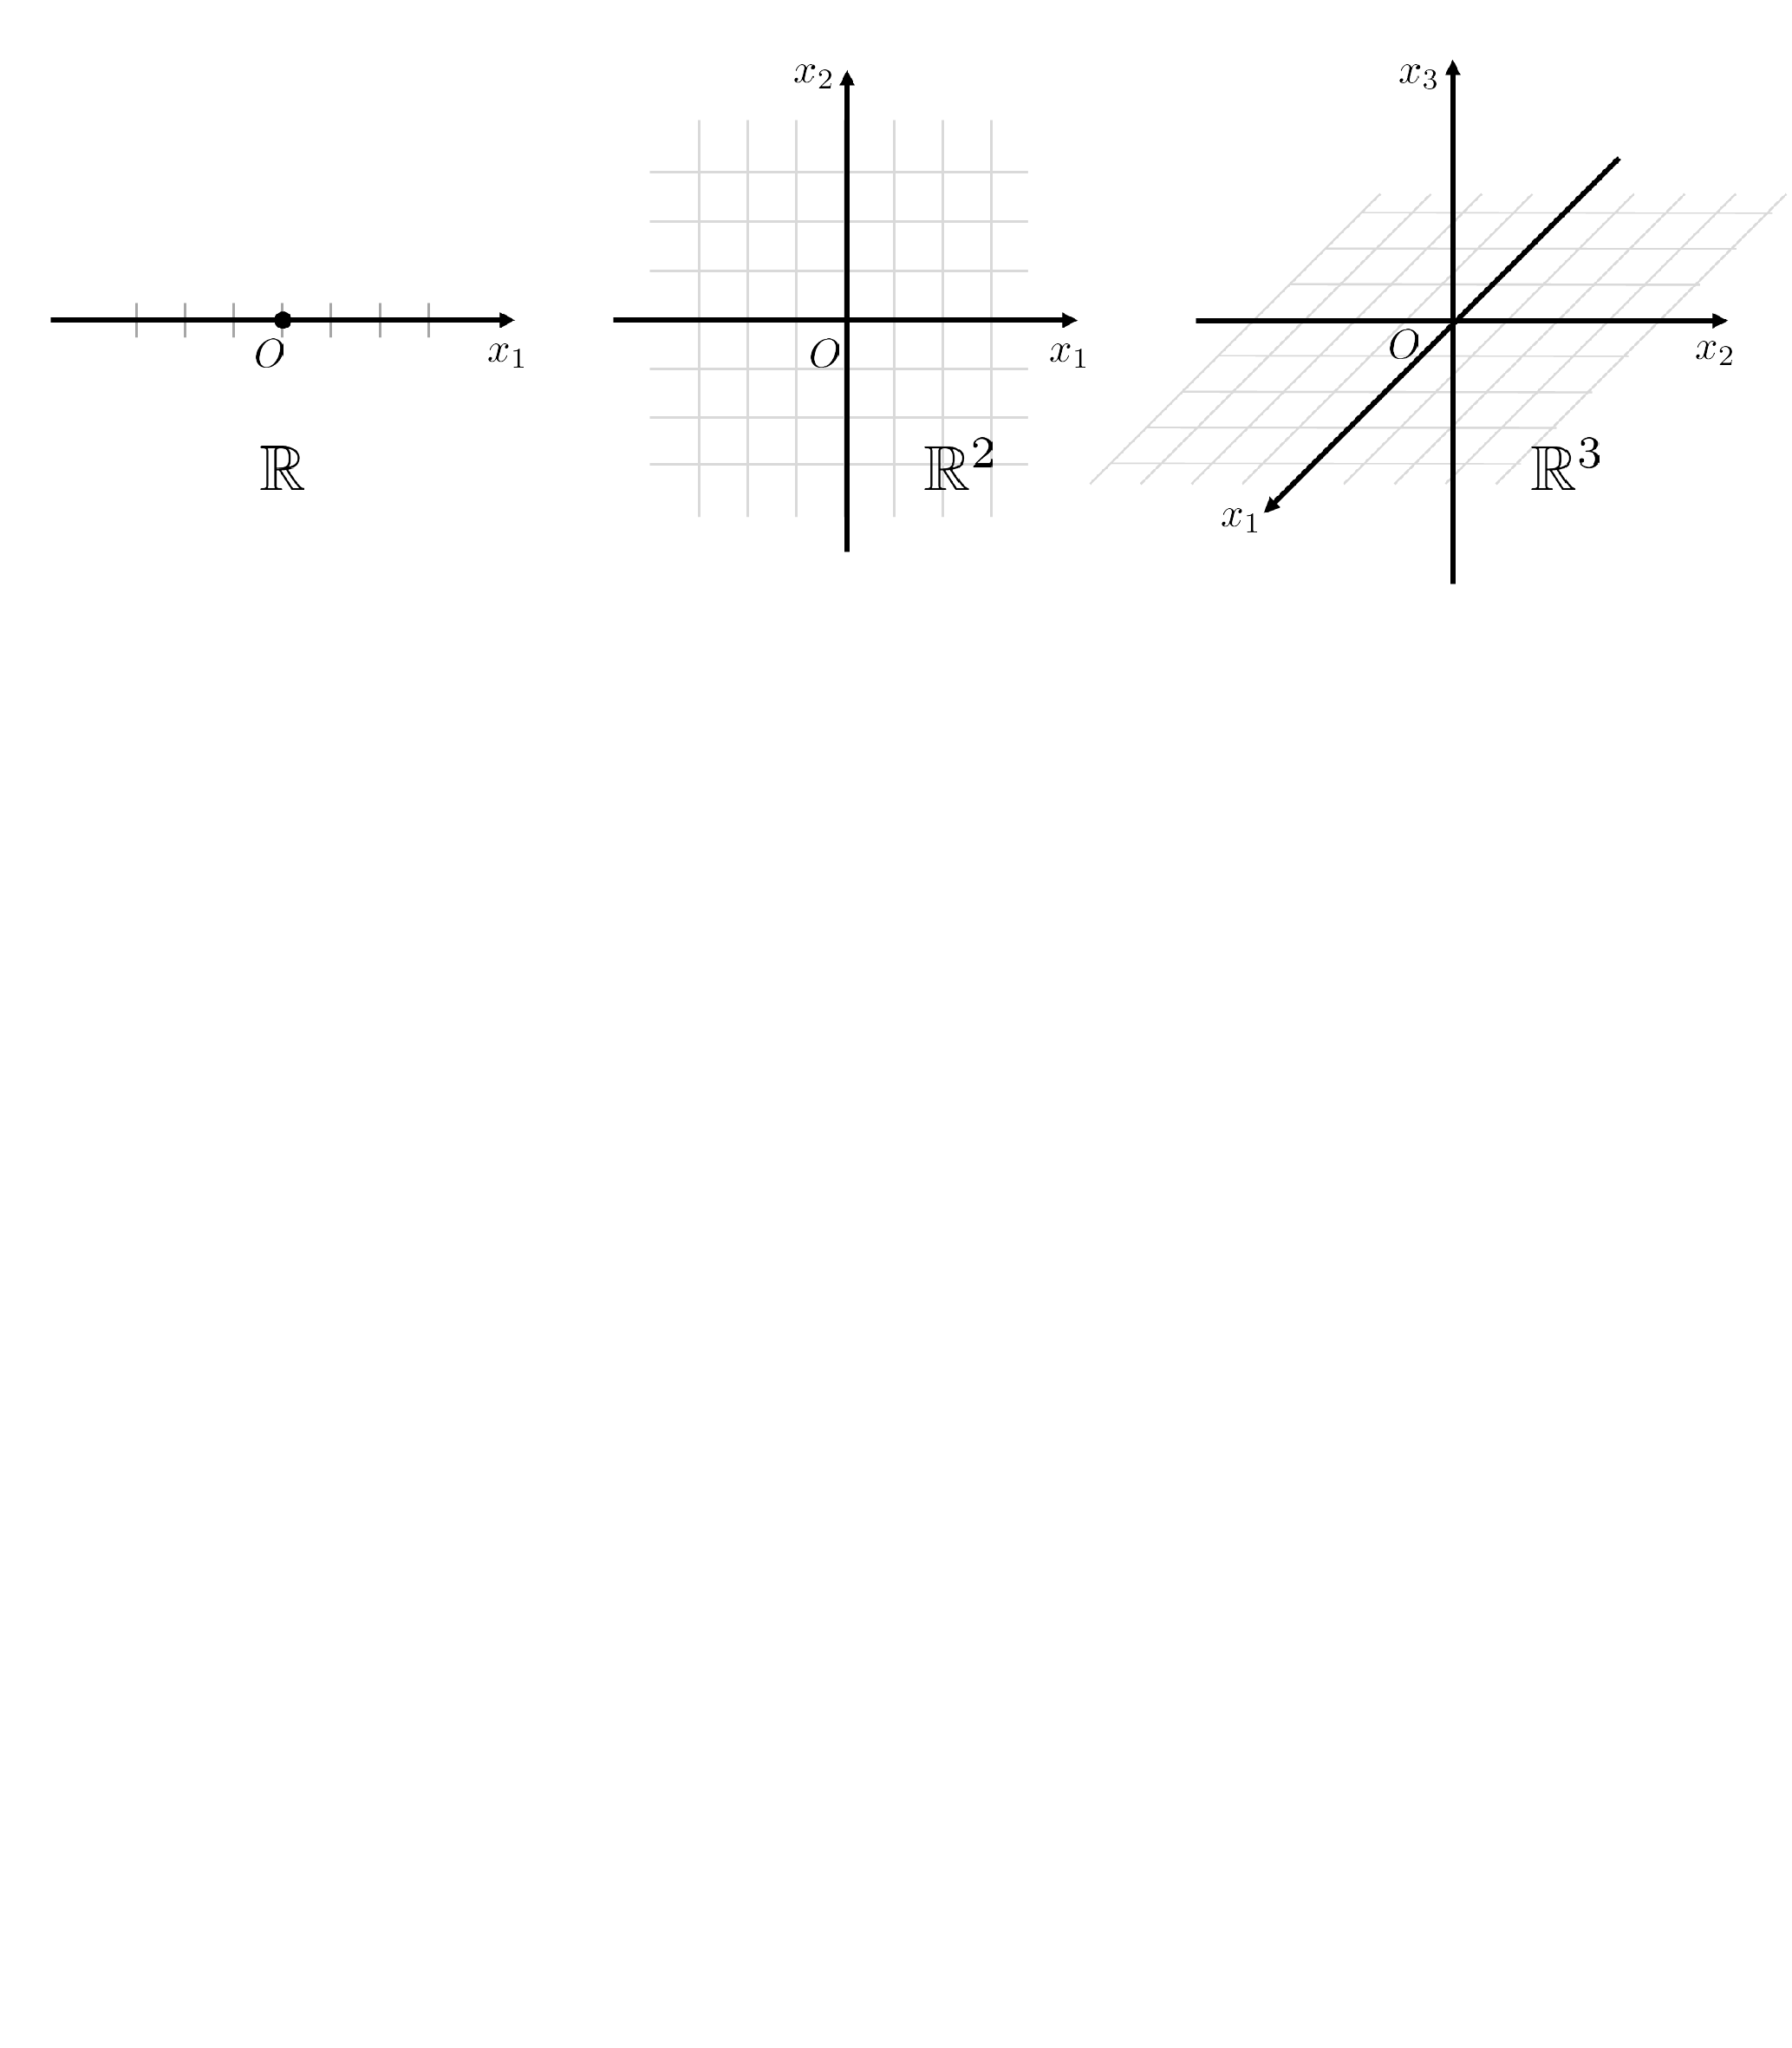
\includegraphics[trim=0 27cm 0 0, clip, width=1\textwidth]{fig/fig_R1R2R3.pdf}
    \caption{实向量空间$\mathbb{R},\mathbb{R}^2,\mathbb{R}^3$}
    \label{fig:R1R2R3}
\end{figure}

\medskip


对于向量空间的结构，
我们早就掌握了一种非常简单的方法来刻画它.
在向量空间$\mathbb{K}^n$中，
多个向量$\bm{x}_1, \bm{x}_2 ,\cdots \bm{x}_m$可以进行\textbf{线性组合}，
从而\textbf{线性表示}出另外一个向量$\bm{x} = k_1\bm{x}_1 + k_2\bm{x}_2 + \cdots k_m \bm{x}_m$.
我们希望从$\mathbb{K}^n$中找出一组最基本的向量，
只用它们就可以唯一地线性表示出$\mathbb{K}^n$中的一切向量.
这样的向量组称为$\mathbb{K}^n$的\textbf{基}.
\medskip
我们重申对它的$2$条要求，
作为定义：

\textit{(1)~~$\mathbb{K}^n$中的一切向量都能由这个向量组线性表示.}

\textit{(2)~~上述线性表示的方法总是唯一的. 这等价于，这个向量组中任何一个向量都不能由其他向量线性表示（此时称这组向量是线性无关的）.}\medskip

基的选择可以很自由.
举例来说，
$\mathbb{R}^3$中的$\bm{i} = (1,0,0),\bm{j} = (0,1,0),\bm{k} = (0,0,1)$是我们最熟悉的一组基，
它构成了笛卡尔坐标系.
$\mathbb{R}^3$的任意向量$\bm{x} = (x_1,x_2,x_3)$可以如下分解，
从而获得它在这组基下的\textbf{坐标}：
\begin{eq1}
    &\bm{x} = (x_1,x_2,x_3) = x_1  \cdot \bm{i} + x_2 \cdot \bm{j} + x_3 \cdot \bm{k}  \\[6pt]
    ~~\Longleftrightarrow
    ~~&\bm{x} = (x_1 , x_2 ,x_3) ~\text{在}~ \{ \bm{i} ,\bm{j} ,\bm{k}  \}\text{~下的坐标是}~(x_1,x_2,x_3)
    \end{eq1}


与此同时，
$\bm{i} = (1,0,0),\bm{j} = (0,1,0),\bm{k}_1 = (1,2,1)$
这$3$个向量也是$\mathbb{R}^3$的一组基（容易验证它满足定义中的$2$个条件）.
$\mathbb{R}^3$的任意向量$(x_1,x_2,x_3)$可以如下分解，并获得它在这组基下的坐标：
\begin{eq1}
    &\bm{x} = (x_1,x_2,x_3) = (x_1-x_3) \cdot \bm{i} + (x_2-2x_3) \cdot \bm{j} + x_3 \cdot \bm{k}_1 \\[6pt]
    ~~\Longleftrightarrow
    ~~&\bm{x} = (x_1 , x_2 ,x_3) ~\text{在}~ \{ \bm{i} ,\bm{j} ,\bm{k}_1  \}\text{~下的坐标是}~(x_1-x_3,x_2-2x_3,x_3) \end{eq1}

由此看出，
在$\mathbb{K}^n$中，
虽然向量本身和向量的坐标都用数组来表示
（可以认为坐标本身也是$\mathbb{K}^n$中的元素），
但它们是完全不同的概念.
一个向量所对应的数组与它在某组基下的坐标可以不同；
同一个向量在不同基下的坐标也可以是不同的.

\subsubsection{线性子空间}

刚刚提到，
$\mathbb{K}^n$可以被形象地说成是直线、平面、空间等几何对象.
但是反过来说，
$n$维的几何对象不一定用$\mathbb{K}^n$才能研究.
例如，
我们在$\mathbb{R}^3$的空间解析几何中经常研究直线和平面.
下述$\mathbb{R}^3$的子集$V_1$和$V_2$分别描述了一条经过原点的直线和一张经过原点的平面（图\ref{fig:V1V2}）：
\begin{eq1}
    V_1 &= \{ c \cdot \bm{\alpha}_1 ~|~ c \in \mathbb{R}\} ~~~~~~~~
    V_2 &= \{ c_1 \cdot \bm{\alpha}_1 + c_2 \cdot \bm{\alpha}_2  ~|~ c_1,c_2 \in \mathbb{R}\}
    \end{eq1}

\begin{figure}[H] 
    \centering
    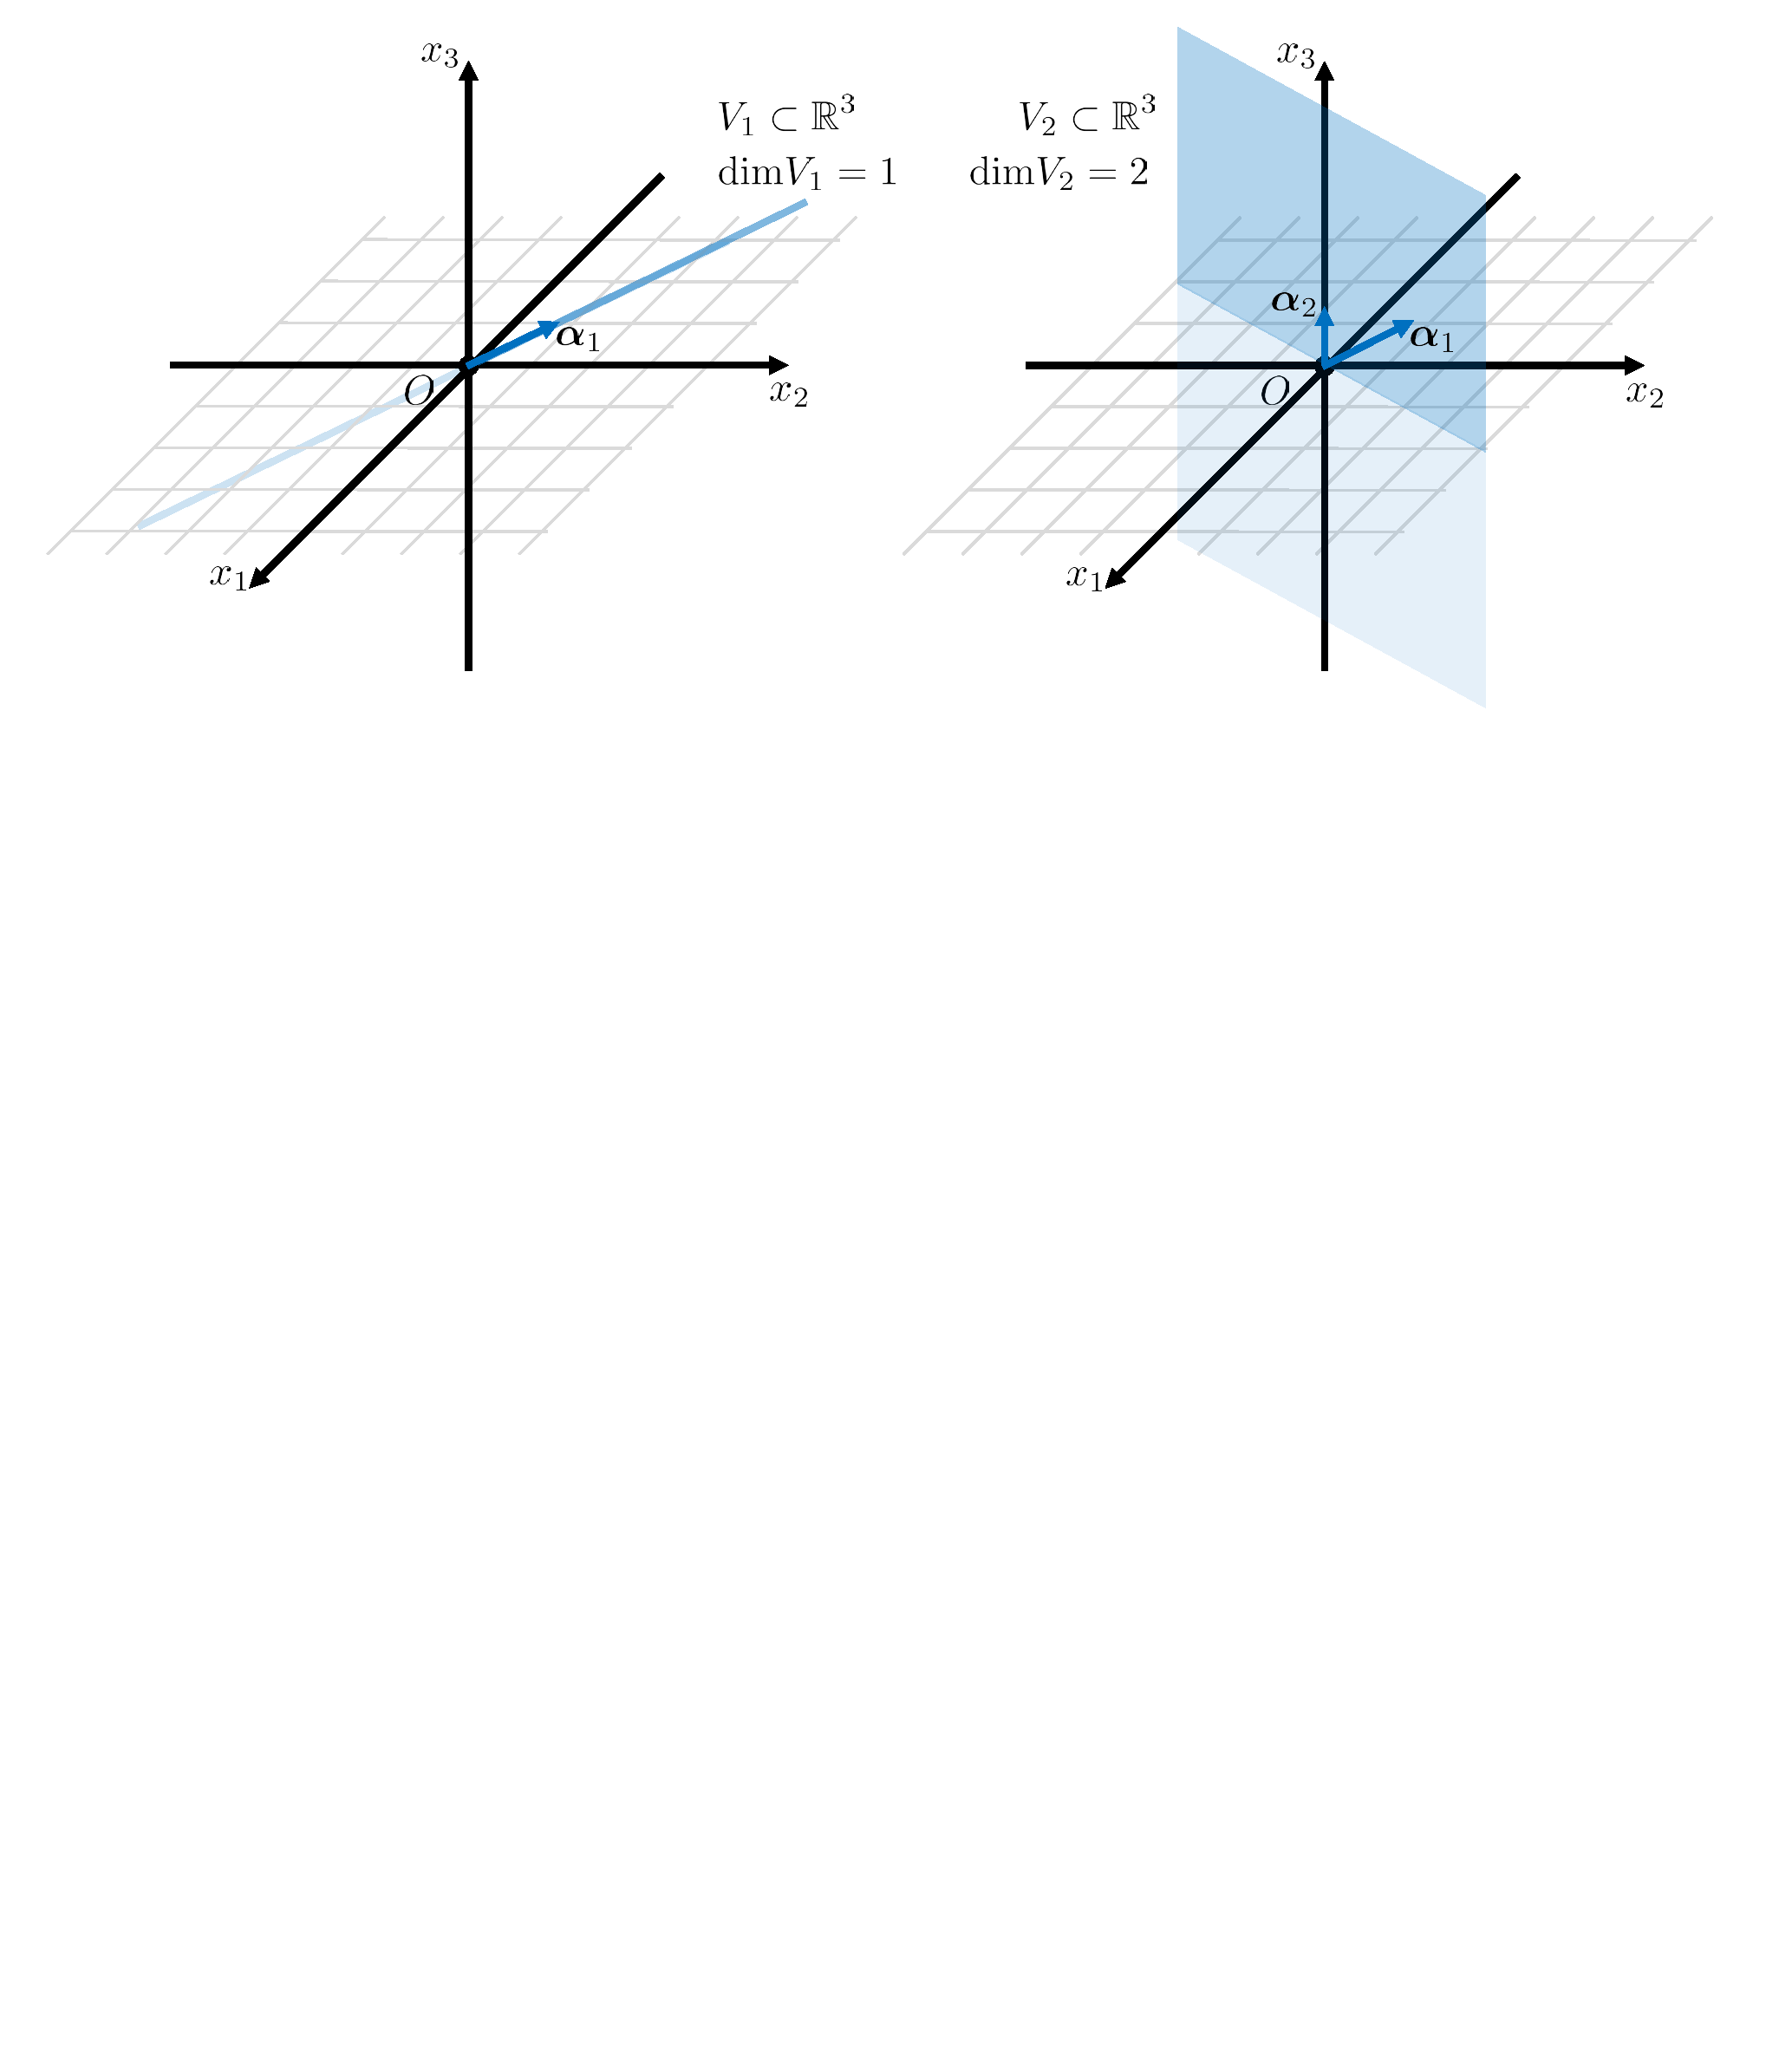
\includegraphics[trim=0 25cm 0 0, clip, width=1\textwidth]{fig/fig_V1V2new.pdf}
    \caption{$\mathbb{R}^3$中的$1$维子空间与$2$维子空间}
    \label{fig:V1V2}
\end{figure}


$V_1$的结构与$\mathbb{R}^1$相同.
这么说有两种含义：
(1)它们都对于向量的加法和数乘封闭，
且向量运算满足之前所述的$8$条性质.
(2)它们都是由$1$个非零向量所能线性表示的所有向量组成的集合.
$V_2$与$\mathbb{R}^2$也可以做类似的比较.
因此，
可以说$V_1,V_2$与向量空间没有本质区别.
但是$V_1$（$V_2$）又不同于$\mathbb{R}^1$（$\mathbb{R}^2$）：
前者事实上是$\mathbb{R}^3$的子集.
我们把这种和向量空间没有本质不同，
但是作为$\mathbb{K}^n$的子集出现的集合，
称为\textbf{$\mathbb{K}^n$的线性子空间}.

根据刚刚的讨论，线性子空间这个概念有两种等价的提法.
第一种：\textit{若$V$是$\mathbb{K}^n$的一个非空子集，且$V$对于向量的加法和数乘运算封闭，则称$V$是$\mathbb{K}^n$的一个线性子空间（简称子空间）.}
第二种：\textit{任取$\mathbb{K}^n$的一个向量组$\bm{\alpha}_1, \bm{\alpha}_2 , \cdots , \bm{\alpha}_s $，
它的所有线性组合构成的集合是$\mathbb{K}^n$的子空间.
称为\textbf{由$\bm{\alpha}_1, \bm{\alpha}_2 , \cdots , \bm{\alpha}_s$生成的子空间}，记作$\langle \bm{\alpha}_1, \bm{\alpha}_2 , \cdots , \bm{\alpha}_s \rangle$}.
向量组$\{\bm{\alpha}_1, \bm{\alpha}_2 , \cdots , \bm{\alpha}_s\}$就是这个子空间的一个\textbf{生成组}.
在此基础上，
如果要求生成组$\{ \bm{\alpha}_1, \bm{\alpha}_2 , \cdots , \bm{\alpha}_s \}$足够精简，
即这个生成组线性无关，
那么$\{ \bm{\alpha}_1, \bm{\alpha}_2 , \cdots , \bm{\alpha}_s \}$
就称为子空间$V$的一组\textbf{基}.
$V$中任意向量$\bm{\beta}$被这组基线性表示的唯一一组系数，
称为$\bm{\beta}$在这组基下的\textbf{坐标}.

有了子空间的定义，
今后再研究向量组的时候，
\textbf{一定要想到它生成的子空间}.
甚至于，
应该用向量组生成的子空间代替向量组本身，
再进行思考.
对于矩阵，
我们会把它看成列向量组或者行向量组，
也就不得不想到它们生成的子空间.
把矩阵列向量组生成的子空间称为\textbf{列空间}，
矩阵行向量组生成的子空间称为\textbf{行空间}.

根据上述定义，
我们容易验证，
$\mathbb{K}^3$中一条过原点的直线和过原点的平面都是子空间，
它们分别可以由$1$个向量和$2$个向量生成，
即基所含向量的个数分别为$1$和$2$.
这两个数契合我们对于“维数”的几何直观：
直线是“$1$维”的，平面是“$2$维”的.
从直观上谈论“维数”这个概念似乎很轻松，
但是为了在数学上能够把握，
有必要对它提出一个严格的定义：
\textit{子空间$V$的一个基所含向量的个数是这个子空间的\textbf{维数}，记作}$\dim V$.
显然，
$\mathbb{K}^n$的$n$维子空间有且仅有一个，也就是它本身.
$\mathbb{K}^n$的$0$维子空间也有且仅有一个，那就是零子空间$\{\bm{0}\}$.

\subsubsection{线性方程组的线性表示（子空间）观点}

从$\mathbb{K}^n$中取向量组$\{ \bm{\alpha}_1 , \bm{\alpha}_2 , \cdots , \bm{\alpha}_s \}$.
再任取$\bm{\beta} \in \mathbb{K}^n$.
由生成子空间的定义知道，
$\bm{\beta}$能由$\{ \bm{\alpha}_1 , \bm{\alpha}_2 , \cdots , \bm{\alpha}_s \}$线性表示，
当且仅当$\bm{\beta} \in \langle \bm{\alpha}_1 , \bm{\alpha}_2 , \cdots , \bm{\alpha}_s \rangle$.
这也等同于说$\bm{\beta}$处在$\{ \bm{\alpha}_1 , \bm{\alpha}_2 , \cdots , \bm{\alpha}_s \}$所确定的直线/平面/空间……中，
是一个比较直观的表述.

同样的事情还可以从线性方程组的角度“翻译”.
考虑如下$s$个未知量，$n$个方程组成的线性方程组$A \bm{x} = \bm{\beta}$：
\begin{eq1}
    \begin{cases}
        a_{11} x_1  + a_{12}x_2 + \cdots + a_{1s} x_s = b_1\\[2pt]
        a_{21} x_1  + a_{22}x_2 + \cdots + a_{2s} x_s = b_2\\[2pt]
        ~\vdots \\[2pt]
        a_{n1} x_1 + a_{n2}x_2 + \cdots + a_{ns} x_s = b_n
    \end{cases} \end{eq1}

其中，$\{ \bm{\alpha}_1 , \bm{\alpha}_2 , \cdots , \bm{\alpha}_s \}$是系数矩阵$A$的列向量组，
$\bm{\beta}$是常数项组成的列向量$ (b_1 , b_2 , \cdots , b_n)$.
那么这个方程组也可以简写成：
\begin{eq1}
    x_1 \bm{\alpha}_1 
    + x_2 \bm{\alpha}_2
    + \cdots 
    + x_s \bm{\alpha}_s 
    =
    \bm{\beta} \end{eq1}

这样就看出来，
\textbf{线性方程组有解等价于$\bm{\beta}$能由$\{ \bm{\alpha}_1 , \bm{\alpha}_2 , \cdots , \bm{\alpha}_s \}$线性表示，
也等价于$\bm{\beta} \in \langle \bm{\alpha}_1 , \bm{\alpha}_2 , \cdots , \bm{\alpha}_s \rangle$.}
因此，
研究方程组有没有解只需要看$\bm{\beta}$和$\langle \bm{\alpha}_1 , \bm{\alpha}_2 , \cdots , \bm{\alpha}_s \rangle$的关系.
进一步地，
在方程组有解的条件下，
如果有唯一解，
意思就是$\bm{\beta}$被$\{ \bm{\alpha}_1 , \bm{\alpha}_2 , \cdots , \bm{\alpha}_s \}$线性表示的方式唯一，
也就是说
$\{ \bm{\alpha}_1 , \bm{\alpha}_2 , \cdots , \bm{\alpha}_s \}$
是
$\langle \bm{\alpha}_1 , \bm{\alpha}_2 , \cdots , \bm{\alpha}_s \rangle$
的一组基，
而方程组的解$(x_1,x_2,\cdots,x_n )$就是$\bm{\beta}$在这组基下的一组坐标.
反之，
方程组有无穷多解.\hypertarget{jie}{}


\subsubsection{线性映射的核空间和像空间}

\hypertarget{ker}{}

现在，我们已经将向量组和线性方程组这两个话题用子空间的语言
统一了起来.
自然，
我们应该把线性映射（矩阵）的某些性质用子空间的语言也“翻译”一遍.

我们知道，
一个线性映射可以写成线性方程组（矩阵乘法）的形式$A \bm{x} = \bm{\beta}$.
从线性映射的角度看，
$\bm{\beta}$是向量$\bm{x}$在线性映射$A$之下的\text{像}.
我们把线性映射$A$的所有像的集合称为\textbf{像空间}，
记作$\operatorname{Im}A$——
为什么用上了“空间”这两个字？
当然是因为\textbf{任何线性映射的像空间都是$\mathbb{K}^n$的一个子空间}.
对此的证明只是简单应用一下线性映射的定义：
如果$A \bm{x}_1 = \bm{\beta}_1 ,~ A \bm{x}_2 = \bm{\beta}_2 $，
那么有$A (\bm{x}_1 + \bm{x}_2) = \bm{\beta}_1 + \bm{\beta}_2,~ A (k\bm{x}_1) = k\bm{\beta}_1$.
这样就从“$\bm{\beta}_1, \bm{\beta}_2 \in \operatorname{Im} A$”推出了
“$\bm{\beta}_1+\bm{\beta}_2,k\bm{\beta}_1 \in \operatorname{Im}A$”，
也就证明了$\operatorname{Im}A$对向量的加法和数乘封闭.

有刚才线性方程组的观点，
我们就可以这样“翻译”$\operatorname{Im}A$：
它是矩阵$A$的列空间，
也是使线性方程组$A \bm{x} = \bm{\beta}$有解的所有$\bm{\beta}$的集合.


在解方程组的时候，
我们一般是固定$\bm{\beta}$，
而去研究$\bm{x}$的集合，
也就是线性方程组的\textbf{解集}.
有趣的是，
我们从解集中也能找到子空间的结构.
考虑线性方程组$A \bm{x} = \bm{0}$.
如果你把它当成线性方程组看，
它是一个齐次线性方程组，
而所有满足方程的$\bm{x}$组成的集合称为齐次线性方程组的\textbf{解空间}，
一般用字母$W$表示——
这里又用到了“空间”这两个字，
表明\textbf{齐次线性方程组的解集是$\mathbb{K}^n$的线性子空间.}
理由如下：
如果向量$\bm{x}_1$和$\bm{x}_2$都是$A \bm{x} = 0$的解，
那么$\bm{0} = A\bm{x}_1 + A\bm{x}_2 = A(\bm{x}_1 + \bm{x}_2)$；
设$k \in \mathbb{K}$，$\bm{0} = k A \bm{x}_1 = A (k\bm{x}_1)$.
即$\bm{x}_1 + \bm{x}_2$和$k \bm{x}_1$也是它的解.
因此，
\textbf{解空间$W$对于向量的加法和数乘运算封闭.}

同样的事情，
切换到线性映射的视角来看可以这样说：
解空间$W$其实就是这样的一些向量的集合，
它们在线性映射$A$下的像都是零向量.
从线性映射的角度赋予这同一个集合新的说法：
$W$其实是零向量$\bm{0}$在线性映射$A$下的\textbf{原像集}，
叫做线性映射$A$的\textbf{核}或者\textbf{核空间}，
记作$\operatorname{Ker}A$.
实际上，
对于一般的线性方程组$A \bm{x} = \bm{\beta}$，
它的解集就是$\bm{\beta}$在线性映射$A$下的\textbf{原像集}.
只不过当$\bm{\beta} \ne \bm{0}$时，
原像集（解集）不是子空间.

我们以$\mathbb{R}^2$上的$5$类基本的线性变换为例，
说明$\operatorname{Im}A$和$\operatorname{Ker}A$的直观意义.
对于旋转、反射、剪切和伸缩，
容易知道它们的核空间是$\{ \bm{0} \}$，
而像空间是整个$\mathbb{R}^2$.
而平行投影变换$P$则不同（图\ref{fig:ImKerP}）.
它的像空间$\operatorname{Im}P = \langle \bm{\alpha}_1 , \bm{\alpha}_2 \rangle = \{ c \cdot \bm{\alpha}_1 ~|~ c \in \mathbb{R}\}$
即是整个$x_1$轴.
于是$\dim\operatorname{Im}P = 1$.
解线性方程组$P\bm{x} = \bm{0}$，
可知$\bm{\eta} = (-\cot \theta , 1)$是一个解，
且$\operatorname{Ker}P = \{ c \cdot \bm{\eta} ~|~ c \in \mathbb{R}\}$，
$\dim\operatorname{Ker}P = 1$.
由此看出，
Im表征了$\mathbb{R}^2$被“拍扁”之后的形状和维数，
Ker表征了$\mathbb{R}^2$被“拍扁”的方向和维数.
可以发现一个重要的数量关系
$n = \dim\operatorname{Ker}A + \dim\operatorname{Im}A$，
其中$n$是全空间的维数（\hyperlink{ex1.2}{例1.2}中有更多例子）.
这个公式称为\textbf{维数公式}，
表明整个空间的维数$n$可以按线性映射$A$分解成核和像两部分的维数之和.
我们将在第二章详细探讨这个事实.

\begin{figure}[H] 
    \centering
    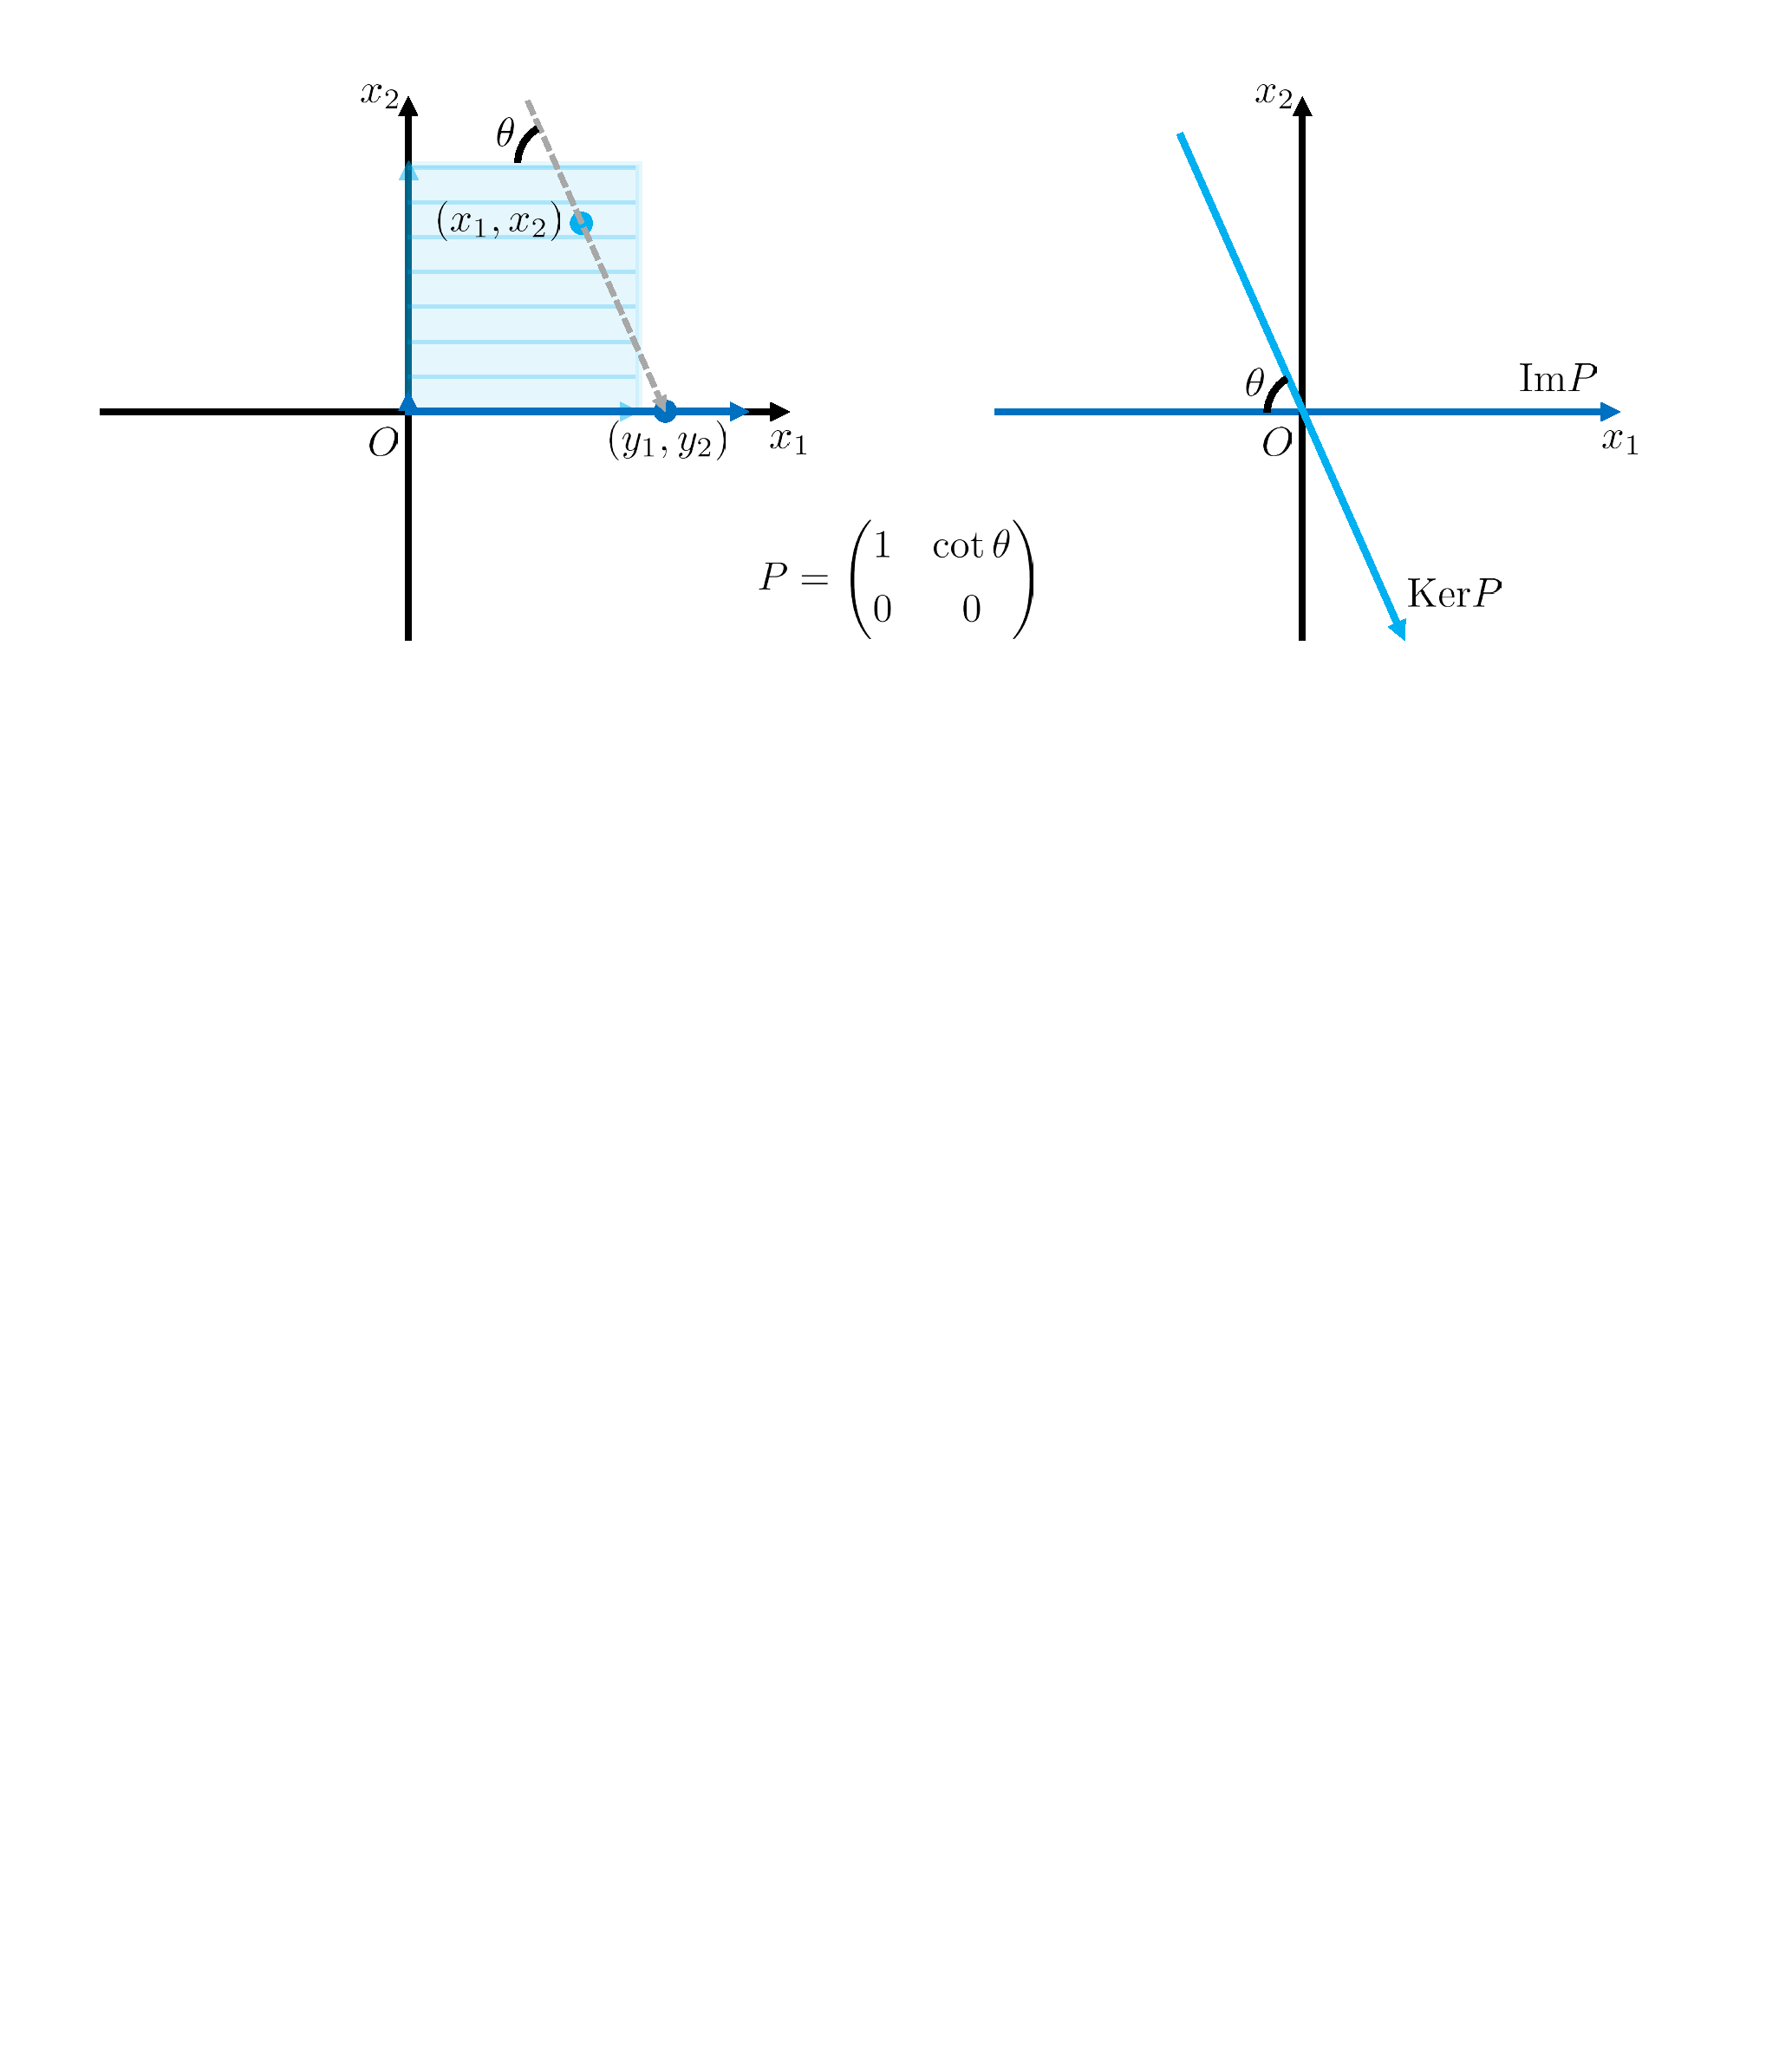
\includegraphics[trim=0 27cm 0 0, clip, width=1\textwidth]{fig/fig_ImKerP.pdf}
    \caption{平行投影变换$P$的核空间和像空间}
    \label{fig:ImKerP}
\end{figure}


到目前为止，
我们讲了许多线性代数所涉及的基本概念.
如果你手中有一本线代教材，
可能会发现有些概念在书中靠后的章节才会提及，
例如线性映射和子空间的知识.
但它们恰是线性代数的精华，
无论从理解还是从解题的角度来说，
都应该最先学习它们，
然后带着它们去攻略别的知识.

除了这些必要工具之外，
我还想总结一下学习线性代数的方法论.
第一是借助具体例子和图像来理解概念，
例如我们多次“请出”$\mathbb{R}^2$上$5$类基本的线性变换来讨论.
第二是灵活地在线性映射（线性变换）、矩阵、线性方程组、向量组和子空间之间进行转换，
把同样的事情借助不同的概念翻来覆去地说.
这种做法我称之为“\textbf{翻译}”.
翻译的过程并没有提供多少实质性的数学内容，
它只是对同一个事物从不同角度做出了解释.
例如在本章中，
谈论平行投影变换$P$与其他$4$种变换的区别，
就有好多种不同的说法.
在真正深入线性代数的具体内容之前，
我们就先对这些已有的说法做个总结.

\subsubsection{向量组的线性相关/线性无关}

\textbf{基}的定义中说到，
如果一个向量组是某个空间的一组基，
它必须是线性无关的.
教材中用如下的说法来定义\textbf{线性相关}和\textbf{线性无关}的概念：\medskip

\textbf{$[1]$线性相关/线性无关的定义}~~
\textit{$\mathbb{K}^n$中的向量组$\bm{\alpha}_1 , \bm{\alpha}_2 , \cdots , \bm{\alpha}_s~(s \ge 1)$是线性相关的，
当且仅当有数域$\mathbb{K}$中的一组不全为$0$的系数$k_1 , k_2 , \cdots , k_s$，使得}
\begin{eq1}
    k_1 \bm{\alpha}_1 
    + k_2 \bm{\alpha}_2 
    + \cdots 
    + k_s \bm{\alpha}_s 
    = \bm{0} \end{eq1}
\textit{反之，如果上式成立可以推出系数$k_1 , k_2 , \cdots , k_s$全为$0$，那么称该向量组是线性无关的.}
\medskip

而我们用的是如下的说法：\medskip

[2]\textit{一个向量组线性无关，
当且仅当其中的任何一个向量都无法被其他向量线性表示；
一个向量组线性相关，
当且仅当其中存在一个向量能被其他向量线性表示.}\medskip

如果你需要从向量组线性表示的角度思考问题，
那么教材上的定义[1]定义总是绕不开的，
有必要记住它.
如果你喜爱用子空间的角度思考问题（这正是我推荐的），
那么一定要知道下面的说法：\medskip

[3]\textit{一个向量组线性无关，
当且仅当它生成的子空间的一组基就是它自己，当且仅当它生成的子空间维数等于它的向量个数；
一个向量组线性相关，
当且仅当它不是它所生成的子空间的一组基，当且仅当它生成的子空间维数小于它的向量个数.
}\medskip

[4]
\textit{$A$的列向量组线性无关，
当且仅当}$\dim\operatorname{Im}A$\textit{与$A$的列数相同.}
\textit{$A$的列向量组线性相关，
当且仅当}$\dim\operatorname{Im}A$\textit{小于$A$的列数.}
\medskip

接下来继续说明如何多角度“翻译”这两个概念.
我们自然还可以将它从线性方程组的角度来解读：\medskip

$[5]$\textit{
$A$的列向量组线性无关当且仅当齐次线性方程组$A\bm{x} = 0$只有零解，
$A$的列向量组线性相关当且仅当齐次线性方程组$A\bm{x} = 0$有非零解.}（考虑到方程组可以用线性表示的观点理解，这就是[2]的直接翻译）\medskip


$[6]$
\textit{$A$的列向量组线性无关当且仅当}$\dim \operatorname{Ker}A = 0$\textit{，即}$\operatorname{Ker}A = \{\bm{0}\}$.
\textit{$A$的列向量组线性相关当且仅当}$\dim \operatorname{Ker}A > 0$（这同时也用到了线性映射和子空间的语言）.\medskip


在$n = s$的特殊情形下（即考虑$n$个$n$维向量构成的向量组），
向量组拼成的矩阵$A$是方阵，
也就是$\mathbb{K}^n$上的线性变换.
对此我们能做更多讨论.\medskip

$[7]$
\textit{$n$个$n$维向量线性无关，
等价于它拼成的矩阵可逆，矩阵对应的线性变换可逆；
$n$个$n$维向量线性相关，
等价于它拼成的矩阵不可逆，矩阵对应的线性变换不可逆.}\medskip

你也许觉得这$7$种说法互相转换很神奇，
但它们与“茴字的$4$种写法”类似，
只是一些数学内容稀薄的文字游戏.
不过从解决具体问题的角度说，
我们需要善于转换角度来分析同一个问题，
这时灵活的“翻译”确实是至关重要的.
例如，
在抽象的证明题中，向量组的线性表示可能难以想象，
转化成子空间来思考能帮助迅速理清逻辑并写出证明（\hyperlink{T1.5}{例1.5}，\hyperlink{T1.6}{例1.6}，\hyperlink{T1.7}{例1.7}）.
而针对具体向量组的线性无关/相关的问题，
则必须通过定义或者线性方程组才能把握（\hyperlink{T1.4}{例1.4}）.
如果你不熟悉这些文字游戏，
甚至于你尚且需要深度思考才会相信“这$7$个说法竟然是一样的”，
那就很容易被一些题目混淆视听了.\medskip

\subsection{习题}

\begin{example}
    在$\mathbb{R}^3$中，
    绕$O$点的转动是一个线性变换.

    (1)~~写出代表$\mathbb{R}^3$任意转动的矩阵$R$. 提示：$\mathbb{R}^3$中的任何转动都可以通过依次绕$x_1$轴，$x_2$轴，$x_3$轴三次旋转来实现.

    (2)~~计算$\mathrm{Im}R$和$\mathrm{Ker}R$，并写出它们的维数.
    
    (3)~~分别计算$\bm{e}_1=(1,0,0),\bm{e}_2=(0,1,0),\bm{e}_3=(0,0,1)$在$R$下的像.

    (4)~~写出$R$的逆矩阵$R^{-1}$.
\end{example}
\smallskip
\begin{solution}
    (1)先尝试写出绕$x_1$轴旋转$\psi$角的变换$R_x(\psi)$，
    这个变换保持任何向量的$x_1$分量不动，
    且$x_2$分量与$x_3$分量的变化与$x_1$无关.
    因此该变换具有如下的形式：
    \begin{eq1}
        \begin{cases}
            y_1 = x_1 \\[2pt]
            y_2 = a_{22}x_2 + a_{23}x_3 \\[2pt]
            y_3 = a_{32}x_2 + a_{33}x_3
        \end{cases}
        ~~~
        \Longleftrightarrow
        ~~~~~~
        R_x(\psi) = 
        \begin{pmatrix}
            1 & 0 & 0 \\[2pt]
            0 & a_{22} & a_{23} \\[2pt]
            0 & a_{32} & a_{33} 
        \end{pmatrix} \end{eq1}

    只看方程组的后两行，
    可以看成平面向量$(x_2,x_3)$旋转$\psi$角后成为平面向量$(y_2,y_3)$.
    因此待定的$4$个系数只需套用$\mathbb{R}^2$上的旋转变换.
    即：
    \begin{eq1}
        R_x(\psi) = 
        \begin{pmatrix}
            1 & 0 & 0 \\[2pt]
            0 & \cos \psi & -\sin \psi \\[2pt]
            0 & \sin \psi & \cos \psi 
        \end{pmatrix} \end{eq1}

    同理，可以写出绕 $x_2$ 轴旋转 $\theta$ 角的矩阵以及绕 $x_3$ 轴旋转 $\varphi$ 角的矩阵：
    \begin{eq1}
    R_y(\theta)=
    \begin{pmatrix}
    \cos\theta & 0 & \sin\theta\\[2pt]
    0 & 1 & 0\\[2pt]
    -\sin\theta & 0 & \cos\theta
    \end{pmatrix}\\[12pt]
    R_z(\varphi)=
    \begin{pmatrix}
    \cos\varphi & -\sin\varphi & 0\\[2pt]
    \sin\varphi & \cos\varphi & 0\\[2pt]
    0 & 0 & 1
    \end{pmatrix}\end{eq1}

    因此，$\mathbb{R}^3$ 中任意旋转均可表示为三个基本旋转的复合：
    \begin{eq1}
    R = R_z(\varphi) R_y(\theta) R_x(\psi).
    \end{eq1}

    计算得：
    \begin{eq1}
    R=
    \begin{pmatrix}
    \cos\varphi\cos\theta &
    \cos\varphi\sin\theta\sin\psi-\sin\varphi\cos\psi &
    \cos\varphi\sin\theta\cos\psi+\sin\varphi\sin\psi
    \\[6pt]
    \sin\varphi\cos\theta &
    \sin\varphi\sin\theta\sin\psi+\cos\varphi\cos\psi &
    \sin\varphi\sin\theta\cos\psi-\cos\varphi\sin\psi
    \\[6pt]
    -\sin\theta &
    \cos\theta\sin\psi &
    \cos\theta\cos\psi
    \end{pmatrix}\end{eq1}

    \bigskip

    (2)~
    在绕原点的旋转变换$R$下，
    除了零向量本身以外，
    不会有任何向量被映成零向量.
    因此：
    \begin{eq1}
    \operatorname{Ker}R=\{0\},\qquad
    \dim\operatorname{Ker}R=0
    \end{eq1}
    
    又$R$显然可逆（其逆变换就是逆向旋转），
    因此：
    \begin{eq1}
    \operatorname{Im}R=\mathbb{R}^3,\qquad
    \dim\operatorname{Im}R=3
    \end{eq1}

    (3)~按照矩阵乘法的规则计算即可.
    $R\bm{e}_{1},R\bm{e}_{2},R\bm{e}_3$恰为$R$的$3$个列向量.

    (4)~直接通过线性方程组反解是非常困难的.
    有两种思路：

    I.~构造逆向旋转.
    对于$R = R_z(\varphi) R_y(\theta) R_x(\psi)$，
    其逆应当是反向依次执行三个定轴旋转，
    而对一个定轴旋转取逆变换只需取旋转角的负值即可：
    \begin{eq1}
        R^{-1} = R_x^{-1}(\psi) R_y^{-1}(\theta) R_z^{-1}(\varphi)
        =  R_x(-\psi) R_y(-\theta) R_z (-\varphi)
    \end{eq1}

    \medskip

    II.~$(\bm{e}_1 , \bm{e}_2 , \bm{e}_3)$是一组单位正交基，
    则它旋转之后的$(R\bm{e}_1 , R\bm{e}_2 , R\bm{e}_3)$也是一组单位正交基，
    也就是说$R$的列向量组是一组单位正交基.
    则它有以下性质：
    \begin{eq1}
        (R\bm{e}_i)^T R\bm{e}_j
        = 
        \begin{cases}
            1, \quad i = j \\[2pt]
            0, \quad i \ne j 
        \end{cases} \end{eq1}

其中$i,j = 1,2,3$.
    可见以$(R\bm{e}_i)^T R\bm{e}_j$为$(i,j)$元的矩阵是$3$阶单位矩阵$I_3$.
    于是根据矩阵乘法的运算规则有
    $R^TR = I_3$，
    即$R$的逆矩阵恰好等于转置矩阵，
    这是线性变换$R$保持向量长度不变的体现，
    具有此性质的矩阵称为\textbf{正交矩阵}.\qed
\end{solution}

\bigskip

\hypertarget{ex1.2}{}
\begin{example}
    ~

    (1)~~写出一个$3$阶实方阵$P$，
    使其对应的线性变换满足$\operatorname{Im}P = \{ (x_1, x_2, x_3) ~|~ x_1 + x_2 + x_3 = 0 \}$.
    计算$\operatorname{Ker}P,\dim\operatorname{Ker}P,\dim\operatorname{Im}P$.

    (2)~~写出一个$3$阶实方阵$Q$，
    使其对应的线性变换满足$\operatorname{Im}P = \{ (x_1, x_2, x_3) ~|~ x_1 = x_2 = x_3 \}$.
    计算$\operatorname{Ker}Q,\dim\operatorname{Ker}Q,\dim\operatorname{Im}Q$.

    (3)~~写出一个$3$阶实方阵$S$，
    使其对应的线性变换满足$\operatorname{Im}S = \{ \bm{0} \}$.
    计算$\operatorname{Ker}S,\dim\operatorname{Ker}S,\dim\operatorname{Im}S$.

\end{example}
\smallskip
\begin{remark}
    注意$\operatorname{Im}A$是$A$的列空间，
    因此只需找到$\operatorname{Im}A$的一个由$3$个向量构成的生成组，
    把它们以列向量的形式拼成矩阵即可.
\end{remark}
\smallskip
\begin{solution}
    （答案不唯一，仅作为示例）

    (1)~$x_1 + x_2 + x_3 = 0$是以$(1,1,1)$为法向量的平面，
    任取两个垂直于它的线性无关向量就能生成它，
    例如$(1,-1,0)$和$(1,0,-1)$.
    于是我们发现$\dim\operatorname{Im}P = 2$.
    再加一个零向量，
    以列向量的形式拼成矩阵：
    \begin{eq1}
        P =
        \begin{pmatrix}
            1 & 1 & 0 \\[2pt]
            -1 & 0 & 0 \\[2pt]
            0 & -1 & 0 
        \end{pmatrix} \end{eq1}
    
    这就是我们要的矩阵$P$.
    计算$\operatorname{Ker}P$即是计算线性方程组$P\bm{x} = \bm{0}$的解集.
    经过计算可得$\operatorname{Ker}P = \langle (0,0,1) \rangle$，
    从而$\dim\operatorname{Ker}P = 1$.

    \medskip

    (2)~$\operatorname{Im}Q = \langle (1,1,1) \rangle$，
    $\dim\operatorname{Im}Q = 1$.
    矩阵$Q$可以是：
    \begin{eq1}
        Q =
        \begin{pmatrix}
            1 & 0 & 0 \\[2pt]
            1 & 0 & 0 \\[2pt]
            1 & 0 & 0 
        \end{pmatrix} \end{eq1}

    解线性方程组$Q\bm{x} = \bm{0}$得$\operatorname{Ker}Q = \langle (0，1，0) , (0,0,1)\rangle$，
    $\dim\operatorname{Ker}Q = 2$.

    \medskip

    (3)~$S$是零矩阵$O$.
    $\operatorname{Ker}S = \mathbb{R}^3$,
    $\dim\operatorname{Ker}S =3$，
    $\dim\operatorname{Im}S = 0$. \qed
\end{solution}
\smallskip
\begin{example}
    对于映射$A: \mathbb{R}^n \to \mathbb{R}^m$，
    我们给出过三种线性映射概念的表述：

    a. $A\bm{0} = \bm{0}$；$A$保持点的共线关系以及距离比例.

    b. $A$的表达式是线性方程组（矩阵乘法）.

    c. $A \bm{x}_1 + A \bm{x}_2 = A(\bm{x}_1 + \bm{x}_2)$；
    $kA\bm{x} = A(k\bm{x}),~\bm{x}_1,\bm{x}_2 , \bm{x} \in \mathbb{R}^n , k \in \mathbb{R}$.

    证明三者是等价的.
\end{example}
\smallskip
\begin{pf}
    $a \Rightarrow c$：
    $a$的后一个条件可以翻译为：
    对任意$\bm{x},\bm{y} \in \mathbb{R}^n$和$k_1,k_2$，有：
    \begin{eq1}
        k_2 (A(\bm{x} + k_1 \bm{y}) - A\bm{x}) = 
        k_1 (A(\bm{x} + k_2 \bm{y}) - A\bm{x})
    \end{eq1}
    
    在该式中令$\bm{x} = \bm{0}$，
    $k_2 = 1$，
    并利用$A\bm{x} = \bm{0}$，
    就得到$A$与数乘有交换性：$A(k_1\bm{y}) = k_1 A\bm{y}$.
    于是，该式又可改写为：
    \begin{eq1}
        A(k_2\bm{x} + k_1k_2 \bm{y}) - A(k_2 \bm{x}) &= 
        A(k_1\bm{x} + k_1k_2 \bm{y}) - A(k_1 \bm{x}) \\[4pt]
        A(k_2\bm{x} + k_1k_2 \bm{y}) &= 
        A(k_1\bm{x} + k_1k_2 \bm{y}) + A((k_2 - k_1)\bm{x}) \end{eq1}

    令$\bm{z}_1 = k_1 \bm{x} + k_1k_2\bm{y}$，
    $\bm{z}_2 = (k_2 - k_1)\bm{x}$.
    则$\bm{z}_1,\bm{z}_2$可以取遍$\mathbb{R}^n$中的向量，
    代入后得到$A(\bm{z}_1 + \bm{z}_2) = A\bm{z}_1 + A\bm{z}_2$.
    \medskip

    $c \Rightarrow a$：
    根据线性性质，$A\bm{0} = A(\bm{0} + \bm{0}) = A\bm{0} + A\bm{0}$，
    因此$A\bm{0} = \bm{0}$.
    另外容易验证$k_2 (A(\bm{x} + k_1 \bm{y}) - A\bm{x}) = 
        k_1 (A(\bm{x} + k_2 \bm{y}) - A\bm{x})$
    是正确的.
    \medskip

    $b \Rightarrow c$：
    $A$写成$m \times n$矩阵$A = (a_{ij})$，
    $\bm{x} = (x_1, x_2, \cdots ,x_n) \in \mathbb{R}^n$
    和$\bm{y} = (y_1, y_2, \cdots ,y_n) \in \mathbb{R}^n$
    写成$n \times 1$矩阵（列向量）.
    则$A\bm{x} + A\bm{y} \in \mathbb{R}^m$的第$i$个分量按照矩阵运算规则计算为：
    \begin{eq1}
        \sum_{j=1}^{m} a_{ij}x_{j1}
        + \sum_{j=1}^{m} a_{ij}y_{j1}
        =
        \sum_{j=1}^{m} a_{ij}(x_{j1}+y_{j1})\end{eq1}
    即$A(\bm{x}+\bm{y})$的第$j$分量.
    而$kA\bm{x}$的第$j$分量计算为：
    \begin{eq1}
        k \sum_{j=1}^{m} a_{ij}x_{j1}
        = \sum_{j=1}^{m} a_{ij} (kx_{j1}) \end{eq1}
    即$A(k\bm{x})$的第$j$分量.
    因此$A(\bm{x}+\bm{y}) = A\bm{x} + A\bm{y}$，
    $kA\bm{x} = Ak\bm{x}$.
    \medskip

    $c \Rightarrow b$：
    取$\mathbb{R}^n$的标准正交基
    $\bm{e}_1 = (1,0,\cdots , 0), \bm{e}_2 = (0,1,0,\cdots 0),\cdots , \bm{e}_n = (0,0,\cdots, 1)$.
    则任意向量$\bm{x} = (x_1 , x_2 , \cdots , x_n) \in \mathbb{R}^n$可以表示为
    $\bm{x} = x_1\bm{e}_1 + x_2 \bm{e}_2 + \cdots + x_n \bm{e}_n$.

    设$A\bm{e}_i = \bm{\alpha}_i = (a_{1i},a_{2i},\cdots , a_{mi}) \in \mathbb{R}^m$.
    则根据$A$的线性性质有：
    \begin{eq1}
        A\bm{x}
        &= A (x_1\bm{e}_1 + x_2 \bm{e}_2 + \cdots + x_n \bm{e}_n)
        = x_1 A \bm{e}_1 +  x_2 A \bm{e}_2 + \cdots +  x_n A \bm{e}_n \\[4pt]
        &= x_1 \bm{\alpha}_1 + x_2 \bm{\alpha}_2 + \cdots + x_n \bm{\alpha}_n \\[4pt]
        &= \begin{pmatrix}
        a_{11} & a_{12} & \cdots & a_{1n} \\[2pt]
        a_{21} & a_{22} & \cdots & a_{2n} \\[2pt]
        \vdots & \vdots & \ddots & \vdots \\[2pt]
        a_{m1} & a_{m2} & \cdots & a_{mn}
        \end{pmatrix}
        \begin{pmatrix}
            x_1 \\[2pt] x_2 \\[2pt] x_3 \\[2pt] \vdots \\[2pt] x_n
        \end{pmatrix} \end{eq1}

\end{pf}
\smallskip
\begin{example}
    已知$\bm{\alpha}_1,\bm{\alpha}_2,\bm{\alpha}_3,\bm{\alpha}_4$线性无关.
    请问以下的向量组是否线性无关？证明你的结论：

    (1)~~$\bm{\alpha}_1+\bm{\alpha}_2,~ \bm{\alpha}_2+\bm{\alpha}_3,
    ~\bm{\alpha}_3+\bm{\alpha}_1$.

    (2)~~$\bm{\alpha}_1+\bm{\alpha}_2, ~\bm{\alpha}_2+\bm{\alpha}_3,~
    \bm{\alpha}_3+\bm{\alpha}_4,~\bm{\alpha}_4+\bm{\alpha}_1$.
\end{example}
\smallskip
\begin{remark}
    对于这种有具体形式的向量组，
    一般得尝试一下用线性无关的定义写成线性方程组，
\end{remark}
\smallskip
\begin{solution}
    (1)~
    该向量组线性无关当且仅当线性方程组
    $x_1(\bm{\alpha}_1+\bm{\alpha}_2)+
     x_2(\bm{\alpha}_2+\bm{\alpha}_3)+
     x_3(\bm{\alpha}_3+\bm{\alpha}_1) = \bm{0}$只有零解.
     整理该方程组得到：
     $(x_1 + x_3)\bm{\alpha}_1
     + (x_1 + x_2)\bm{\alpha}_2
     + (x_2 + x_3)\bm{\alpha}_3 = \bm{0}$.
     因为向量组$\{ \bm{\alpha}_1 , \bm{\alpha}_2 , \bm{\alpha}_3 \}$线性无关，
     根据线性无关的定义得$x_1 + x_2 = x_1 + x_2 = x_2 + x_3 = 0$，
     即$x_1 = x_2 = x_3 = 0$.
     因此题目中的向量组是线性无关的.

     (2)~
     注意到$(\bm{\alpha}_1+\bm{\alpha}_2)
     -(\bm{\alpha}_2+\bm{\alpha}_3)
    +(\bm{\alpha}_3+\bm{\alpha}_4)
    -(\bm{\alpha}_4+\bm{\alpha}_1) = \bm{0}$，
    因此是线性相关的.
    
    （如果不幸没能注意到，
    也可以仿照第(1)问的做法建立线性方程组，
    但这一次发现方程组有非零解.）\qed
\end{solution}

\bigskip

接下来的几个有关向量组的问题，
均从子空间的角度给予解答.
当然，
使用向量组和线性方程组的知识也是可以的，
最终殊途同归.
我认为从子空间的角度来思考最简单也最优雅，
而教材因为编排顺序的关系，
几乎没有展示此类思路.
我们通过这几道题以及后续章节的部分题目予以补充.
这三道题目证得的命题也是非常实用的，
今后还会回顾和使用它们
（安全起见，
教材上未出现的命题在考试中使用应当先予以证明）.


\bigskip

\hypertarget{T1.5}{}
\begin{example}
    考虑数域$\mathbb{K}$上的$n$个方程的$n$元线性方程组
    \begin{eq1}
        x_1 \bm{\alpha}_1 + x_2 \bm{\alpha}_2+ \cdots + x_n \bm{\alpha}_n = \bm{\beta} \end{eq1}

    (1)~该方程组对任何
    $\bm{\beta} \in \mathbb{K}^n$
    都有解的充分必要条件是它系数矩阵$A$的列向量组线性无关.

    (2)~该方程组若有解则只有唯一解的充分必要条件也是它系数矩阵$A$的列向量组线性无关.
\end{example}
\smallskip
\begin{pf}
    (1)~
    线性方程组$x_1 \bm{\alpha}_1 + x_2 \bm{\alpha}_2+ \cdots + x_n \bm{\alpha}_n = \bm{\beta}$
    对任何$\bm{\beta} \in \mathbb{K}^n$都有解

    $\Longleftrightarrow$
    对任意的$\bm{\beta} \in \mathbb{K}^n$
    有$\bm{\beta} = \langle \bm{\alpha}_1 , \bm{\alpha}_2, \cdots, \bm{\alpha}_n \rangle$
    
    $\Longleftrightarrow$
    $\mathbb{K}^n \subset \langle \bm{\alpha}_1 , \bm{\alpha}_2, \cdots, \bm{\alpha}_n \rangle$
    
    $\Longleftrightarrow$
    $\mathbb{K}^n = \langle \bm{\alpha}_1 , \bm{\alpha}_2, \cdots, \bm{\alpha}_n \rangle$
    
    $\Longleftrightarrow$
    $\dim\langle \bm{\alpha}_1 , \bm{\alpha}_2, \cdots, \bm{\alpha}_n \rangle = n$.
    
    $\Longleftrightarrow$
    $\{\bm{\alpha}_1 , \bm{\alpha}_2, \cdots, \bm{\alpha}_n\}$，即$A$的列向量组线性无关.

    \medskip

    (2)~
    $A$的列向量组线性无关
    
    $\Longleftrightarrow$
    线性变换$A$可逆

    $\Longleftrightarrow$
    $\bm{x} = A^{-1}\bm{\beta}$一定是该方程组的唯一解.
\end{pf}

注：从线性映射的角度看，
本题第(1)问的条件可以翻译为
“线性变换$A$是满射”，
本题第(2)问的条件可以翻译为
“线性变换$A$是单射”，
而证得的结论可以翻译为
“线性变换$A$是可逆映射，即双射”.
可见\textbf{对于线性变换来说，
满射、单射与双射是等价的.}
从简单的推理中我们就得到了如此奇妙且重要的结论.

\bigskip

\hypertarget{T1.6}{}
\begin{example}
    证明：$\mathbb{K}^n$中任意$n+1$个向量都线性相关.
\end{example}
\smallskip
\begin{pf}
    $n+1$个向量能生成的最大空间是$\mathbb{K}^n$，
    即$n$维空间，
    因此$n+1$一定小于生成子空间的维数，
    向量组一定线性相关.
\end{pf}

\bigskip

\hypertarget{T1.7}{}
\begin{example}
    证明：设向量组$\{\bm{\alpha}_1 , \bm{\alpha}_2 , \cdots , \bm{\alpha}_s  \}$线性无关.
则$\bm{\beta}$能被它线性表示当且仅当$\bm{\alpha}_1 , \bm{\alpha}_2 , \cdots , \bm{\alpha}_s, \bm{\beta}$线性相关.
\end{example}
\smallskip
\begin{pf}
    $\bm{\beta}$能被向量组$\{\bm{\alpha}_1 , \bm{\alpha}_2 , \cdots , \bm{\alpha}_s  \}$线性表示

    $\Longleftrightarrow$
    $\bm{\beta} \in \langle \bm{\alpha}_1 , \bm{\alpha}_2 , \cdots , \bm{\alpha}_s  \rangle$

    $\Longleftrightarrow$
    $\langle \bm{\beta} , \bm{\alpha}_1 , \bm{\alpha}_2 , \cdots , \bm{\alpha}_s  \rangle 
    = \langle \bm{\alpha}_1 , \bm{\alpha}_2 , \cdots , \bm{\alpha}_s  \rangle$

    $\Longleftrightarrow$
    $\dim\langle \bm{\alpha}_1 , \bm{\alpha}_2 , \cdots , \bm{\alpha}_s, \bm{\beta}  \rangle 
    =\dim \langle \bm{\alpha}_1 , \bm{\alpha}_2 , \cdots , \bm{\alpha}_s  \rangle
    =s < s+1$ （利用线性无关性）

    $\Longleftrightarrow$
    $\{\bm{\alpha}_1 , \bm{\alpha}_2 , \cdots , \bm{\alpha}_s, \bm{\beta} \}$线性无关. 
    （$\dim \langle \bm{\alpha}_1 , \bm{\alpha}_2 , \cdots , \bm{\alpha}_s ,\bm{\beta} \rangle$要么是$s$，
    要么是$s+1$.）
\end{pf}
